\documentclass[12pt]{article}

\usepackage[T2A]{fontenc}
\usepackage[utf8]{inputenc}
\usepackage[russian]{babel}
\usepackage{amsmath, amssymb}
\usepackage{graphicx}
\usepackage{booktabs}
\usepackage[a4paper, margin=1.8cm]{geometry}
\usepackage{float}
\usepackage{hyperref}
\usepackage{multirow}
\usepackage{adjustbox}

\hyphenpenalty=10000
\sloppy

\graphicspath{{../results/figures/}}

\begin{document}

\begin{titlepage}
    \begin{center}
        
\includegraphics[width=0.3\textwidth]{img/ifmologo.png}\\[0.5cm]
        \textbf{Университет ИТМО}\\[0.3cm]
        Факультет ИТиП\\
        Группа M3232\\[2cm]

        {\Large \textbf{Лабораторная работа №5}}\\[0.5cm]
        {\large Задача регрессии}\\[0.5cm]
        Дисциплина: Методы оптимизации\\[3cm]

        \begin{flushright}
            Выполнили:\\
            Дегтярев Александр Сергеевич\\
            Надточий Ярослав Вадимофич\\[1cm]
            Проверила: Матвеева М.В.\\
        \end{flushright}

        \vfill
        Санкт-Петербург, 2025
    \end{center}
\end{titlepage}

\tableofcontents
\newpage

%=============================================================================
\section{Постановка задачи}

Исследуется задача восстановления регрессионной зависимости по зашумлённым данным. Данные генерируются на основе аналитических функций:
\[
    y_i = f_{\text{true}}(x_i) + \xi_i, \quad \xi_i \sim \mathcal{N}(0, \sigma^2).
\]

\subsection*{Наборы данных}

Сгенерированы два набора по $m = 150$ точек каждый:

\begin{enumerate}
    \item \textbf{Почти линейная зависимость} (almost\_linear):
    \[
        f_{\text{true}}(x) = 2x - 1 + 0.1\sin(4x), \quad x \in [-3, 3], \quad \sigma = 0.25.
    \]

    \item \textbf{Сильно нелинейная зависимость} (nonlinear):
    \[
        f_{\text{true}}(x) = 0.5x^3 - x + \sin(3x) + 2\exp\!\big({-10(x-1)^2}\big), \quad x \in [-2, 2], \quad \sigma = 0.3.
    \]
\end{enumerate}

\subsection*{Модели регрессии}

Полиномиальная регрессия степеней $p \in \{1, 2, 3, 4, 5\}$. Для $p=1$~--- линейная регрессия. Матрица признаков $\Phi$ содержит мономы $1, x, x^2, \ldots, x^p$. Входной признак $x$ нормализуется перед построением степеней для уменьшения числа обусловленности.

\subsection*{Функции потерь}

Эмпирический риск (MSE) и четыре варианта функции потерь:
\[
    \mathcal{L}(w) = \underbrace{\frac{1}{m}\sum_{i=1}^{m}(\hat{y}_i - y_i)^2}_{Q(w)} + \lambda_1 \|w\|_1 + \lambda_2 \|w\|_2^2,
\]
где $\hat{y}_i = \Phi_i w$. Варианты: без регуляризации ($\lambda_1 = \lambda_2 = 0$), L1 ($\lambda_1 > 0$), L2 ($\lambda_2 > 0$), Elastic Net ($\lambda_1, \lambda_2 > 0$). Для свободного коэффициента регуляризация не применяется.

\subsection*{Оптимизаторы}

\begin{enumerate}
    \item Аналитическое решение задачи линейной регрессии через оценки средних (для $p = 1$);
    \item Стохастический градиентный спуск (SGD, batch\_size = 1);
    \item Mini-batch градиентный спуск (batch\_size = 32);
    \item Метод Гаусса--Ньютона;
    \item Метод Гаусса--Ньютона с регуляризацией Левенберга--Марквардта.
\end{enumerate}

Для каждого метода сохраняется история значений функции потерь, эмпирического риска и регуляризационных слагаемых. Для SGD и mini-batch фиксируются размер batch, число эпох и правило выбора шага.

%=============================================================================
\section{Теоретические основы}

\subsection{Задача наименьших квадратов}

Полиномиальная регрессия сводится к задаче наименьших квадратов: для матрицы признаков $\Phi \in \mathbb{R}^{m \times (p+1)}$ и вектора наблюдений $y \in \mathbb{R}^m$ найти вектор коэффициентов $w$, минимизирующий $Q(w) = \frac{1}{m}\|\Phi w - y\|^2$. Приравняв градиент к нулю, получаем нормальные уравнения $\Phi^T \Phi w = \Phi^T y$. Решение единственно, когда $\Phi^T\Phi$ обратима (столбцы $\Phi$ линейно независимы).

\subsection{Проблема обусловленности}

Матрица $\Phi$ содержит столбцы $1, x, x^2, \ldots, x^p$. При больших $p$ столбцы становятся почти линейно зависимыми, и число обусловленности $\kappa(\Phi^T\Phi)$ растёт экспоненциально. Например, при $p=10$ без нормализации $\kappa \sim 3 \cdot 10^7$. Большое $\kappa$ означает:
\begin{itemize}
    \item малые изменения в данных вызывают большие изменения в $w$;
    \item итеративные методы сходятся медленно;
    \item решение нормальных уравнений теряет точность из-за ошибок округления.
\end{itemize}

\textbf{Нормализация} каждого столбца $\Phi$ к нулевому среднему и единичной дисперсии уменьшает $\kappa$ на порядки, стабилизируя все методы.

\subsection{Переобучение и регуляризация}

При высокой степени $p$ полином имеет $p+1$ параметров и может точно пройти через шумные точки, <<запоминая>> шум вместо истинной зависимости. Это \textit{переобучение}: MSE на обучающей выборке мало, но модель плохо обобщается.

Регуляризация добавляет штраф на величину коэффициентов, вынуждая модель выбирать <<простые>> решения:
\begin{itemize}
    \item \textbf{L1 (Lasso):} $\lambda_1 \sum |w_j|$. Штраф пропорционален абсолютным значениям. Геометрически~--- область допустимых $w$ имеет <<углы>> на осях, поэтому оптимальное решение часто лежит на оси (некоторые $w_j = 0$). Это обеспечивает \textit{разреженность}~--- автоматический отбор признаков.
    \item \textbf{L2 (Ridge):} $\lambda_2 \sum w_j^2$. Штраф пропорционален квадратам. Область допустимых $w$~--- шар, решение не обнуляет коэффициенты, а равномерно уменьшает их. L2 также улучшает обусловленность: $\Phi^T\Phi + m\lambda_2 I$ всегда обратима.
    \item \textbf{ElasticNet:} комбинация $\lambda_1 \|w\|_1 + \lambda_2 \|w\|_2^2$. Сочетает разреженность L1 и стабильность L2.
\end{itemize}

Свободный член (intercept $w_0$) не регуляризуется, чтобы не смещать среднее предсказание.

%=============================================================================
\section{Описание методов оптимизации}

\subsection{Аналитическое решение}

Для линейной регрессии ($p=1$) минимум MSE достигается в замкнутой форме:
\[
    a = \frac{\sum (x_i - \bar{x})(y_i - \bar{y})}{\sum (x_i - \bar{x})^2}, \quad b = \bar{y} - a\bar{x}.
\]
Это частный случай решения нормальных уравнений $\Phi^T\Phi w = \Phi^T y$ при $p=1$. Вычисление стоит $O(m)$ и не требует итераций.

\subsection{SGD и Mini-batch GD}

\textbf{Идея.} Вместо вычисления полного градиента по всем $m$ точкам, на каждом шаге используем подмножество (\textit{мини-батч}) $B \subset \{1, \ldots, m\}$:
\[
    \nabla_w \mathcal{L} \approx \frac{2}{|B|} \Phi_B^T(\Phi_B w - y_B) + \lambda_1 \cdot \text{sign}(w) + 2\lambda_2 w.
\]
При $|B| = 1$ (SGD) градиент максимально шумный, но обновления максимально частые. При $|B| = m$ (полный GD) градиент точный, но дорогой.

\textbf{L1 градиент.} Функция $|w_j|$ недифференцируема в нуле. Используется сглаженная аппроксимация: $\text{sign}(w_j) \approx w_j / \sqrt{w_j^2 + \varepsilon}$, $\varepsilon = 10^{-8}$, что обеспечивает непрерывный градиент.

\textbf{Скорость обучения} убывает: $\alpha_t = \alpha_0 / (1 + \gamma t)$, где $\gamma$~--- коэффициент затухания. Убывание необходимо для сходимости: постоянный шаг не позволяет SGD сойтись к точному минимуму (только колеблется вблизи).

\textbf{Gradient clipping.} Если $\|\nabla\| > 100$, градиент масштабируется: $\nabla \leftarrow \nabla \cdot 100 / \|\nabla\|$. Это предотвращает <<взрыв>> обновлений при плохой обусловленности.

\subsection{Метод Гаусса--Ньютона}

\textbf{Идея.} Специализированный метод Ньютона для задачи наименьших квадратов. В общем методе Ньютона нужен полный гессиан $\nabla^2 \mathcal{L}$, который содержит члены с вторыми производными $r_i$. Гаусс--Ньютон аппроксимирует гессиан как $\frac{2}{m}\Phi^T\Phi$, отбрасывая члены второго порядка. Для линейной регрессии эта аппроксимация точна (вторые производные $r_i$ равны нулю), поэтому метод находит оптимум за 1 шаг.

\textbf{Итерация} решает систему нормальных уравнений:
\[
    (\Phi^T\Phi + m\lambda_2 R)\, h = -\Phi^T r - m\lambda_2 R w,
\]
где $r = \Phi w - y$~--- вектор невязок, $R$~--- диагональная матрица регуляризации (нулевой элемент для свободного члена).

\textbf{Сложность итерации:} $O(n^2 m)$ для формирования $\Phi^T\Phi$ и $O(n^3)$ для решения системы. При $m \gg n$ (150 точек, $p \leq 10$) это дёшево. Сходимость квадратичная вблизи решения.

\textbf{Ограничение.} Если $\Phi^T\Phi$ плохо обусловлена, решение системы теряет точность.

\subsection{Метод Левенберга--Марквардта}

\textbf{Идея.} Добавляет демпфирующий член $\mu I$ к матрице нормальных уравнений:
\[
    (\Phi^T\Phi + m\lambda_2 R + \mu I)\, h = -\Phi^T r - m\lambda_2 R w.
\]

\textbf{Интерпретация.} При $\mu \to 0$ метод совпадает с Гаусс--Ньютоном (быстрая локальная сходимость). При $\mu \to \infty$ шаг $h \approx -\frac{1}{\mu}g$~--- малый шаг в направлении антиградиента (медленная, но гарантированная сходимость). Таким образом, LM интерполирует между двумя методами.

\textbf{Адаптация $\mu$.} При успешном шаге (функция уменьшилась): $\mu \to \mu/2$~--- доверяем модели, переходим ближе к Гаусс--Ньютону. При неудачном: $\mu \to 2\mu$~--- уменьшаем шаг, переходим ближе к градиентному спуску. Начальное $\mu_0 = 0.01$.

\textbf{Преимущество.} $\Phi^T\Phi + \mu I$ всегда обратима при $\mu > 0$, даже если $\Phi^T\Phi$ вырождена. Это делает LM устойчивым к плохой обусловленности.

%=============================================================================
\section{Результаты}

\subsection{Наборы данных}

\begin{figure}[H]
\centering
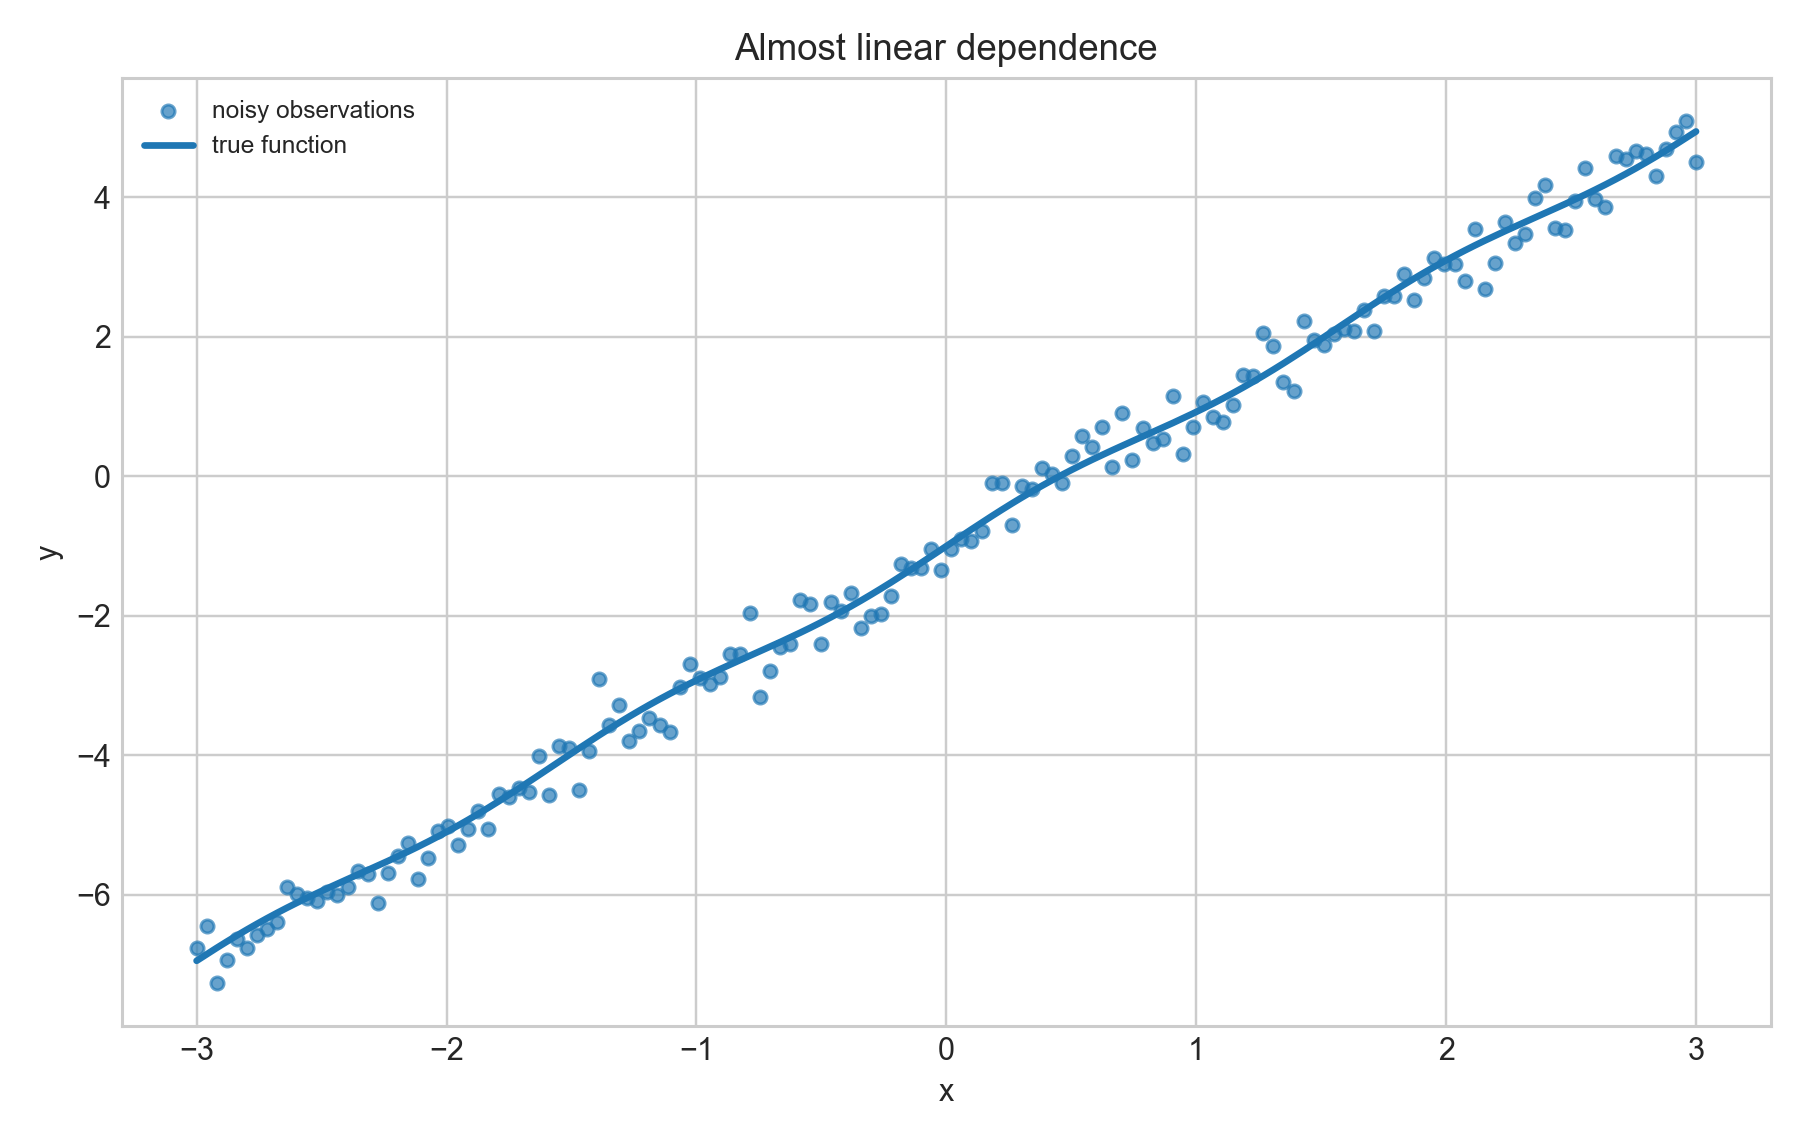
\includegraphics[width=0.48\textwidth]{datasets/almost_linear.png}
\hfill
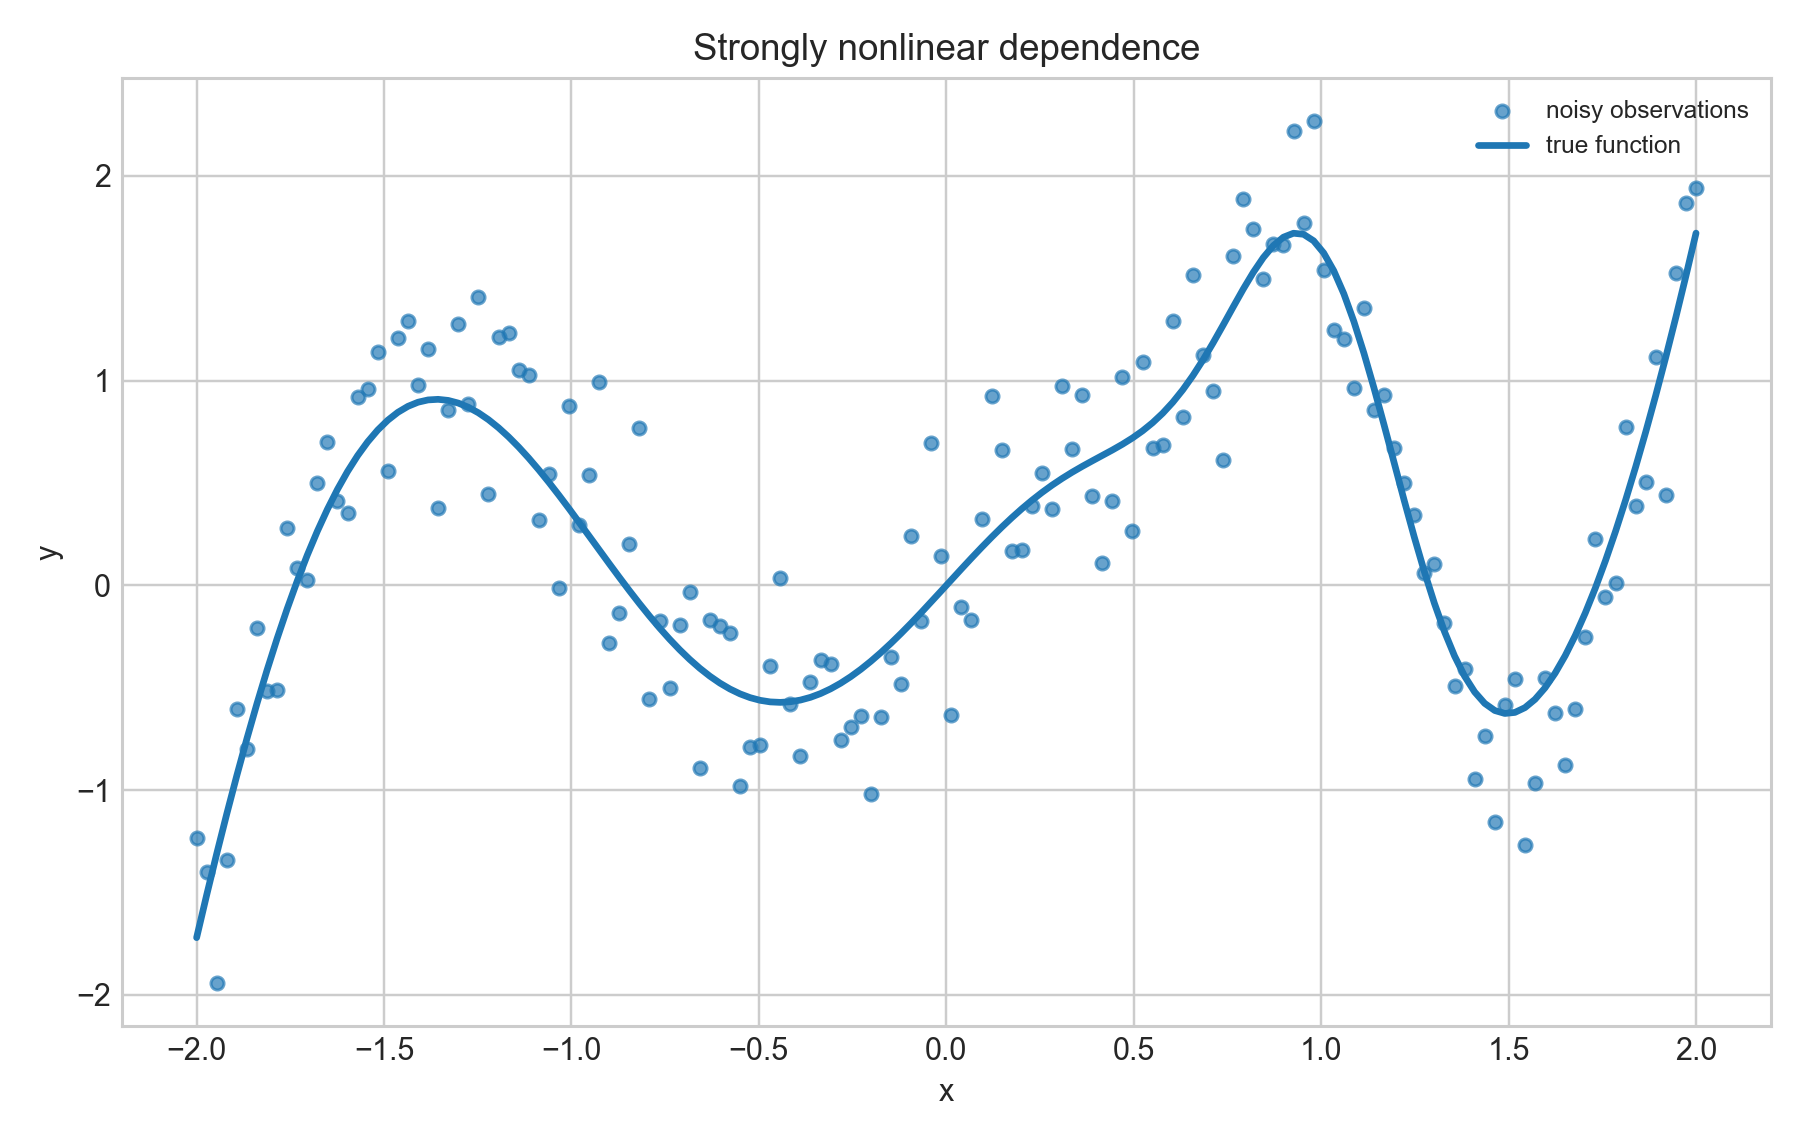
\includegraphics[width=0.48\textwidth]{datasets/nonlinear.png}
\caption{Наборы данных: почти линейный (слева) и нелинейный (справа)}
\end{figure}

\subsection{Базовые модели: сравнение методов оптимизации}

\textbf{Зачем этот эксперимент.} Сравниваем все методы оптимизации на одних и тех же данных и моделях. Для каждой пары <<набор данных + степень полинома>> запускаем все доступные методы и сравниваем: (a)~итоговое MSE (качество аппроксимации), (b)~число итераций/эпох, (c)~число вычислений градиента, (d)~время работы. Ожидаем, что методы второго порядка (GN, LM) сойдутся за единицы итераций, а стохастические (SGD, mini-batch)~--- будут приближаться к оптимуму, но не достигнут его за ограниченное число эпох.

\subsubsection{Набор данных <<almost\_linear>>}

\begin{table}[H]
\centering
\caption{Результаты на наборе almost\_linear}
\begin{adjustbox}{max width=\textwidth}
\begin{tabular}{llccccl}
\toprule
\textbf{Степень} & \textbf{Метод} & \textbf{MSE} & \textbf{Итер./эпохи} & \textbf{$\nabla f$-выч.} & \textbf{Время, с} & \textbf{Статус} \\
\midrule
\multirow{5}{*}{1}
 & Analytic & 0.0812 & 1 & 0 & 0.00004 & closed\_form \\
 & SGD & 0.0812 & 360 & 54000 & 0.707 & max\_epochs \\
 & Mini-batch & 0.0812 & 360 & 1800 & 0.042 & max\_epochs \\
 & Gauss-Newton & 0.0812 & 2 & 2 & 0.0003 & converged \\
 & Lev.-Marq. & 0.0812 & 4 & 4 & 0.0004 & converged \\
\midrule
\multirow{4}{*}{3}
 & SGD & 0.0830 & 360 & 54000 & 1.164 & max\_epochs \\
 & Mini-batch & 0.0816 & 360 & 1800 & 0.062 & max\_epochs \\
 & Gauss-Newton & 0.0803 & 2 & 2 & 0.0003 & converged \\
 & Lev.-Marq. & 0.0803 & 6 & 6 & 0.0006 & converged \\
\midrule
\multirow{4}{*}{5}
 & SGD & 0.0831 & 360 & 54000 & 0.717 & max\_epochs \\
 & Mini-batch & 0.1080 & 360 & 1800 & 0.040 & max\_epochs \\
 & Gauss-Newton & 0.0791 & 2 & 2 & 0.0002 & converged \\
 & Lev.-Marq. & 0.0791 & 6 & 6 & 0.0004 & converged \\
\bottomrule
\end{tabular}
\end{adjustbox}
\end{table}

\subsubsection{Набор данных <<nonlinear>>}

\begin{table}[H]
\centering
\caption{Результаты на наборе nonlinear}
\begin{adjustbox}{max width=\textwidth}
\begin{tabular}{llccccl}
\toprule
\textbf{Степень} & \textbf{Метод} & \textbf{MSE} & \textbf{Итер./эпохи} & \textbf{$\nabla f$-выч.} & \textbf{Время, с} & \textbf{Статус} \\
\midrule
\multirow{5}{*}{1}
 & Analytic & 0.6916 & 1 & 0 & 0.00003 & closed\_form \\
 & SGD & 0.6917 & 360 & 54000 & 0.707 & max\_epochs \\
 & Mini-batch & 0.6916 & 360 & 1800 & 0.035 & max\_epochs \\
 & Gauss-Newton & 0.6916 & 2 & 2 & 0.0001 & converged \\
 & Lev.-Marq. & 0.6916 & 4 & 4 & 0.0003 & converged \\
\midrule
\multirow{4}{*}{3}
 & SGD & 0.6940 & 360 & 54000 & 0.723 & max\_epochs \\
 & Mini-batch & 0.6857 & 360 & 1800 & 0.035 & max\_epochs \\
 & Gauss-Newton & 0.6857 & 2 & 2 & 0.0001 & converged \\
 & Lev.-Marq. & 0.6857 & 5 & 5 & 0.0004 & converged \\
\midrule
\multirow{4}{*}{5}
 & SGD & 0.2390 & 360 & 54000 & 0.712 & max\_epochs \\
 & Mini-batch & 0.3669 & 360 & 1800 & 0.036 & max\_epochs \\
 & Gauss-Newton & 0.2247 & 2 & 2 & 0.0001 & converged \\
 & Lev.-Marq. & 0.2247 & 7 & 7 & 0.0005 & converged \\
\bottomrule
\end{tabular}
\end{adjustbox}
\end{table}

Gauss-Newton сходится за 2 итерации для всех степеней и наборов данных. Levenberg-Marquardt требует 4--25 итераций. SGD и mini-batch не сходятся за 360 эпох, но при малых степенях достигают близких значений MSE.

\begin{figure}[H]
\centering
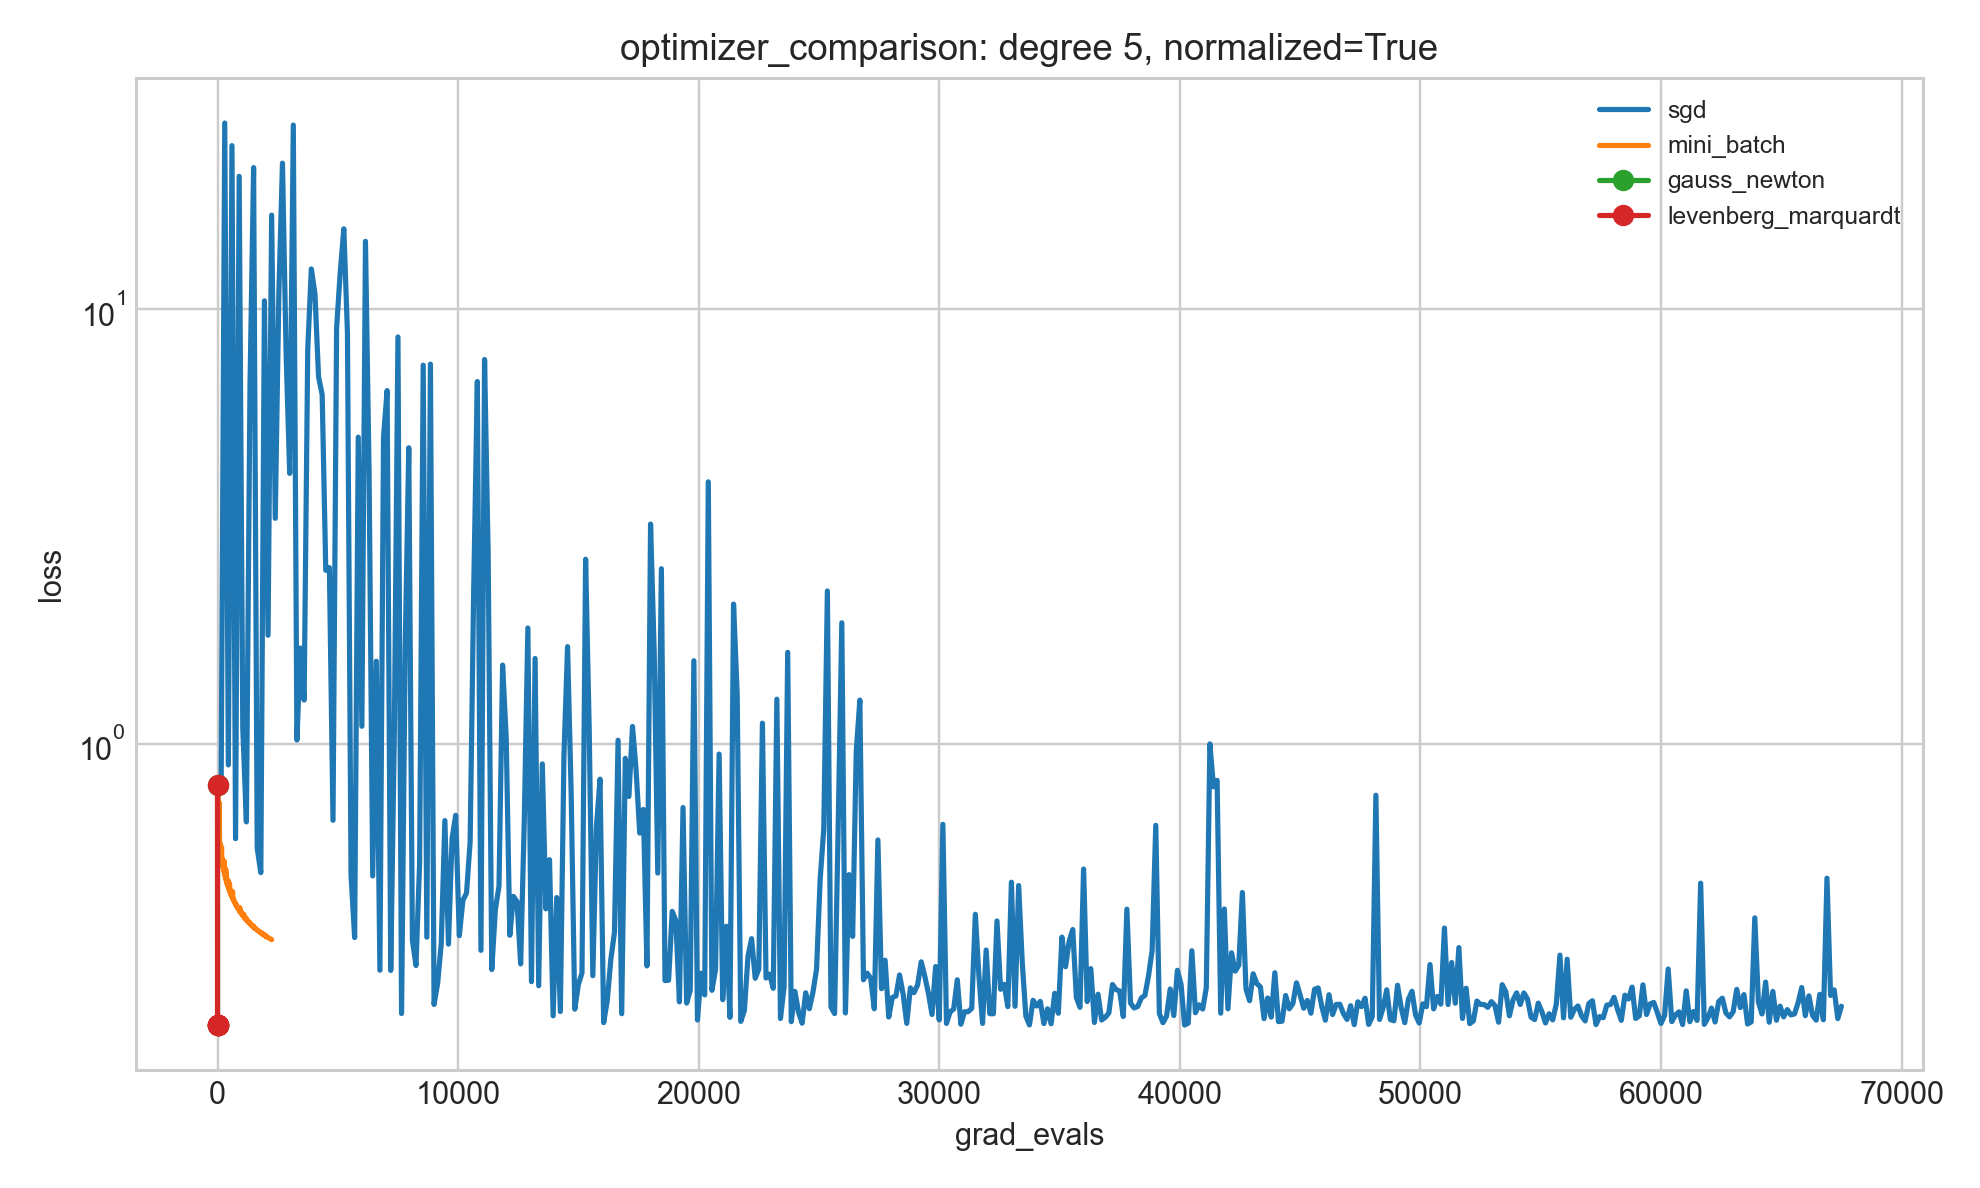
\includegraphics[width=0.85\textwidth]{optimizer_comparison/loss_degree_5_normalized_True.png}
\caption{Сравнение методов: динамика потерь для степени 5}
\end{figure}

\subsubsection{Примеры аппроксимации}

\begin{figure}[H]
\centering

\includegraphics[width=0.48\textwidth]{base_models/nonlinear/degree_1/gauss_newton/fit.png}
\hfill

\includegraphics[width=0.48\textwidth]{base_models/nonlinear/degree_5/gauss_newton/fit.png}
\caption{Аппроксимация нелинейного набора: степень 1 (слева) и степень 5 (справа), Gauss-Newton}
\end{figure}

\begin{figure}[H]
\centering
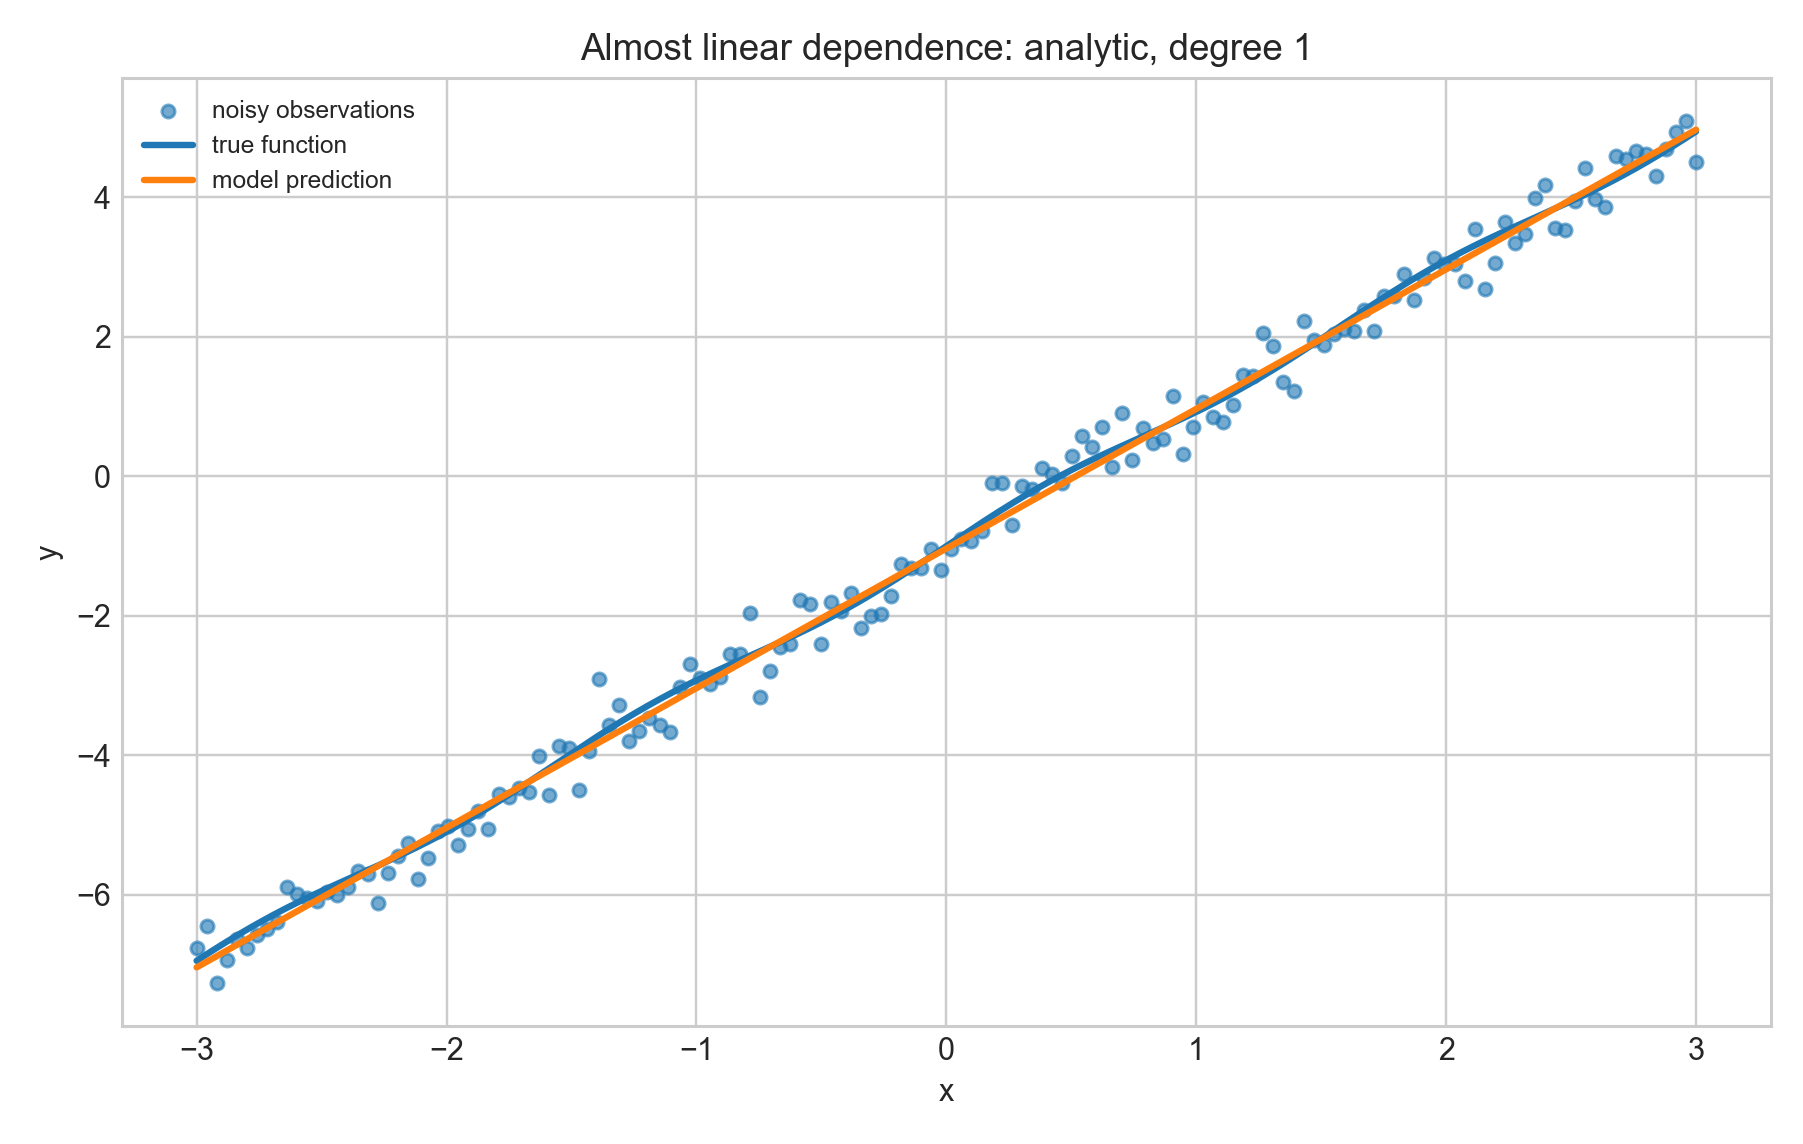
\includegraphics[width=0.48\textwidth]{base_models/almost_linear/degree_1/analytic/fit.png}
\hfill

\includegraphics[width=0.48\textwidth]{base_models/almost_linear/degree_5/gauss_newton/fit.png}
\caption{Аппроксимация линейного набора: степень 1 аналитически (слева) и степень 5 Gauss-Newton (справа)}
\end{figure}

\subsection{Влияние размера батча}

\textbf{Зачем этот эксперимент.} Размер батча $|B|$~--- ключевой гиперпараметр стохастических методов. Он определяет компромисс:
\begin{itemize}
    \item Малый батч~--- больше обновлений за эпоху, но каждое зашумлено (дисперсия градиента $\sim 1/|B|$). Шум помогает <<выбираться>> из плохих областей, но замедляет финальную сходимость.
    \item Большой батч~--- точный градиент, но мало обновлений за эпоху. При фиксированном бюджете эпох модель получает меньше <<опыта>>.
\end{itemize}
Задание требует сравнить размеры 1, 4, 8, 16, 32, 64, 150 ($\approx m$) по скорости сходимости, стабильности и вычислительной эффективности.

Эксперимент на наборе <<nonlinear>> со степенью 5 (достаточно сложная модель для проявления различий). Все конфигурации использовали 480 эпох.

\begin{table}[H]
\centering
\caption{Влияние размера батча на качество (nonlinear, степень 5)}
\begin{tabular}{cccc}
\toprule
\textbf{Batch size} & \textbf{MSE} & \textbf{$\nabla f$-выч.} & \textbf{Время, с} \\
\midrule
1   & 0.2566 & 72\,000 & 0.936 \\
4   & 0.2291 & 18\,240 & 0.250 \\
8   & 0.2332 & 9120   & 0.136 \\
16  & 0.2707 & 4800   & 0.081 \\
32  & 0.3589 & 2400   & 0.048 \\
64  & 0.4331 & 1440   & 0.035 \\
150 & 0.5517 & 480    & 0.037 \\
\bottomrule
\end{tabular}
\end{table}

Малые батчи (4--8) достигают лучшего MSE, но требуют больше вычислений градиента. Большие батчи (64--150) быстрее, но не успевают сойтись за ограниченное число эпох. Оптимальный баланс~--- batch\_size = 4 (MSE = 0.229 при 18\,240 вычислениях градиента).

\begin{figure}[H]
\centering
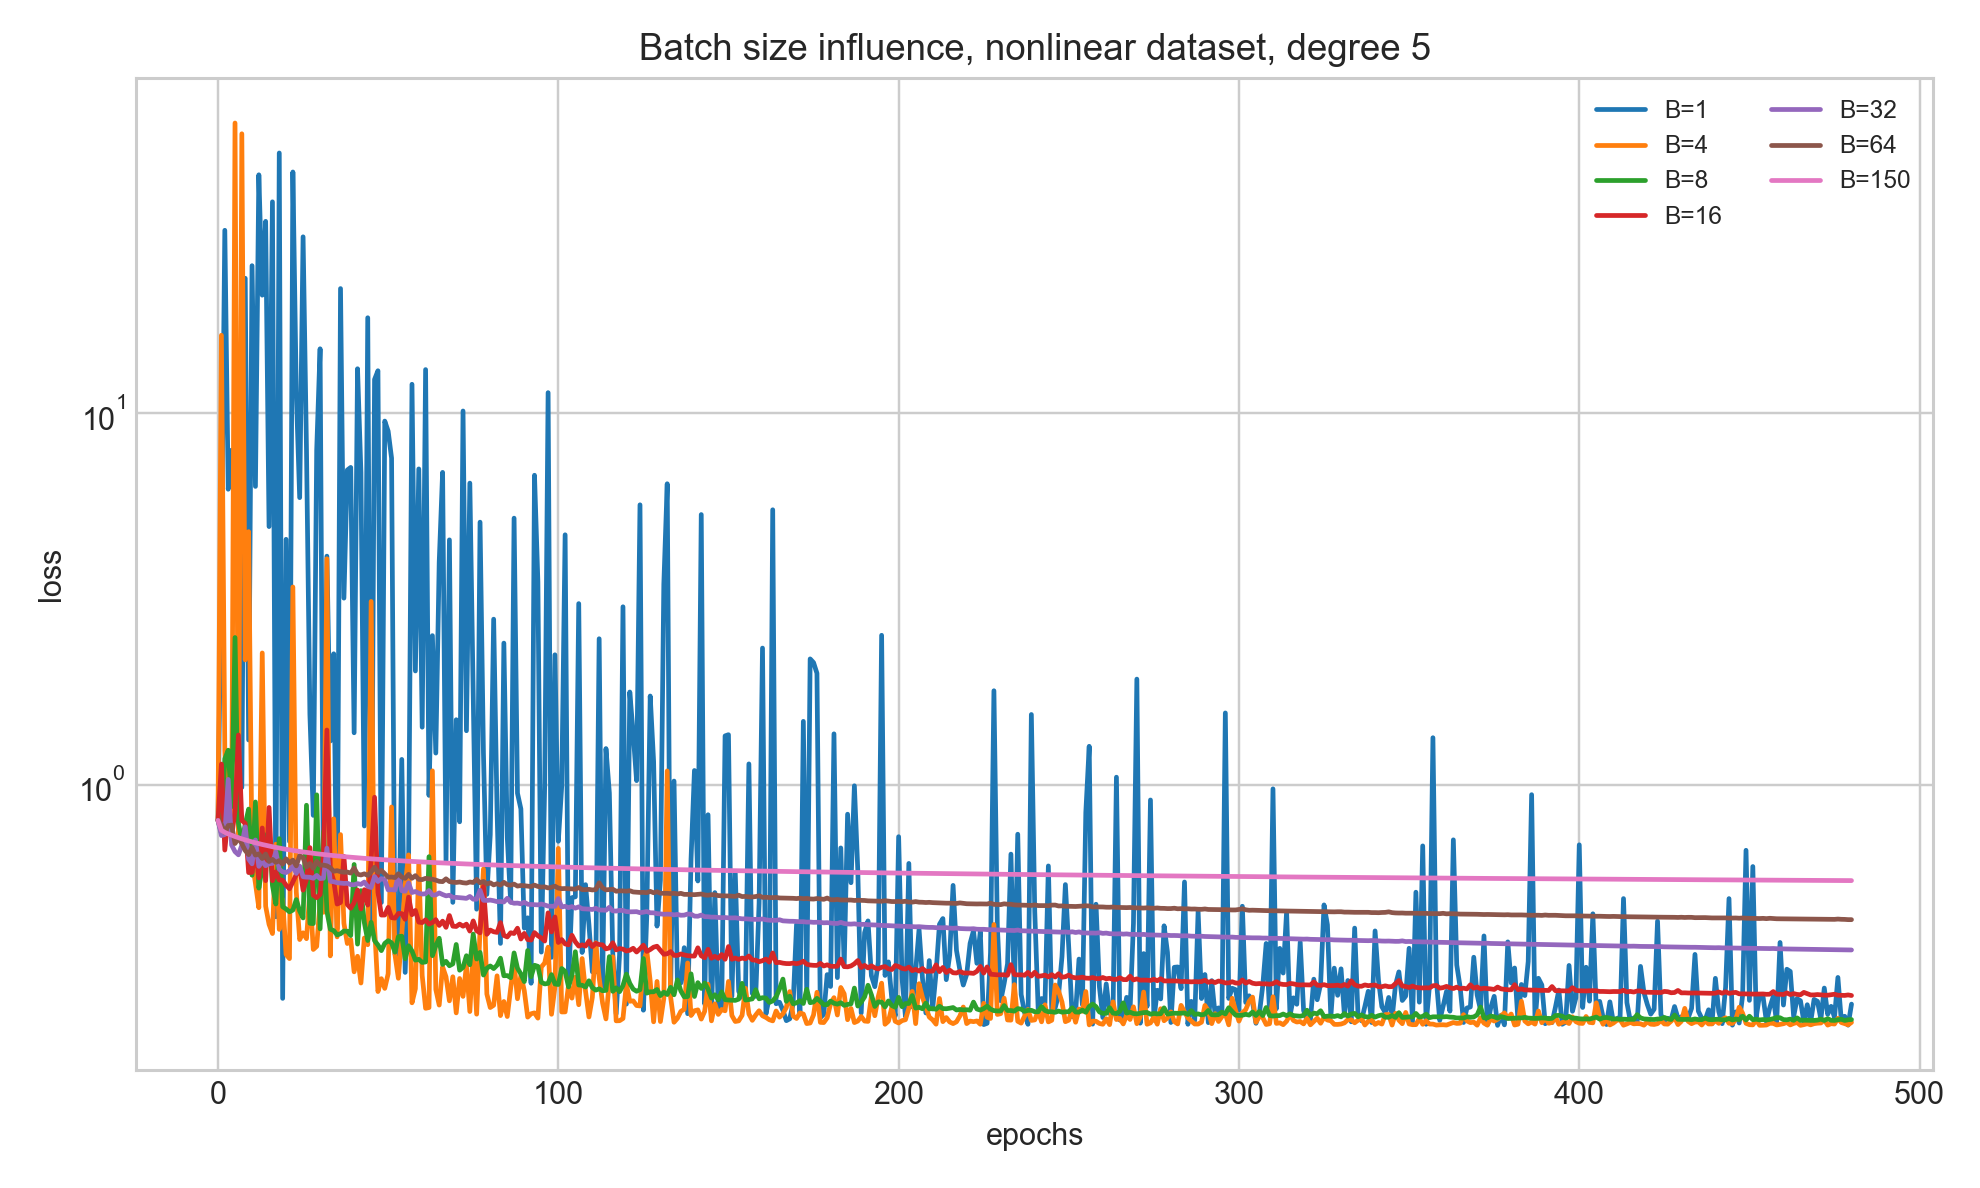
\includegraphics[width=0.85\textwidth]{batch_size/loss_by_epoch.png}
\caption{Потери по эпохам для разных размеров батча}
\end{figure}

\begin{figure}[H]
\centering
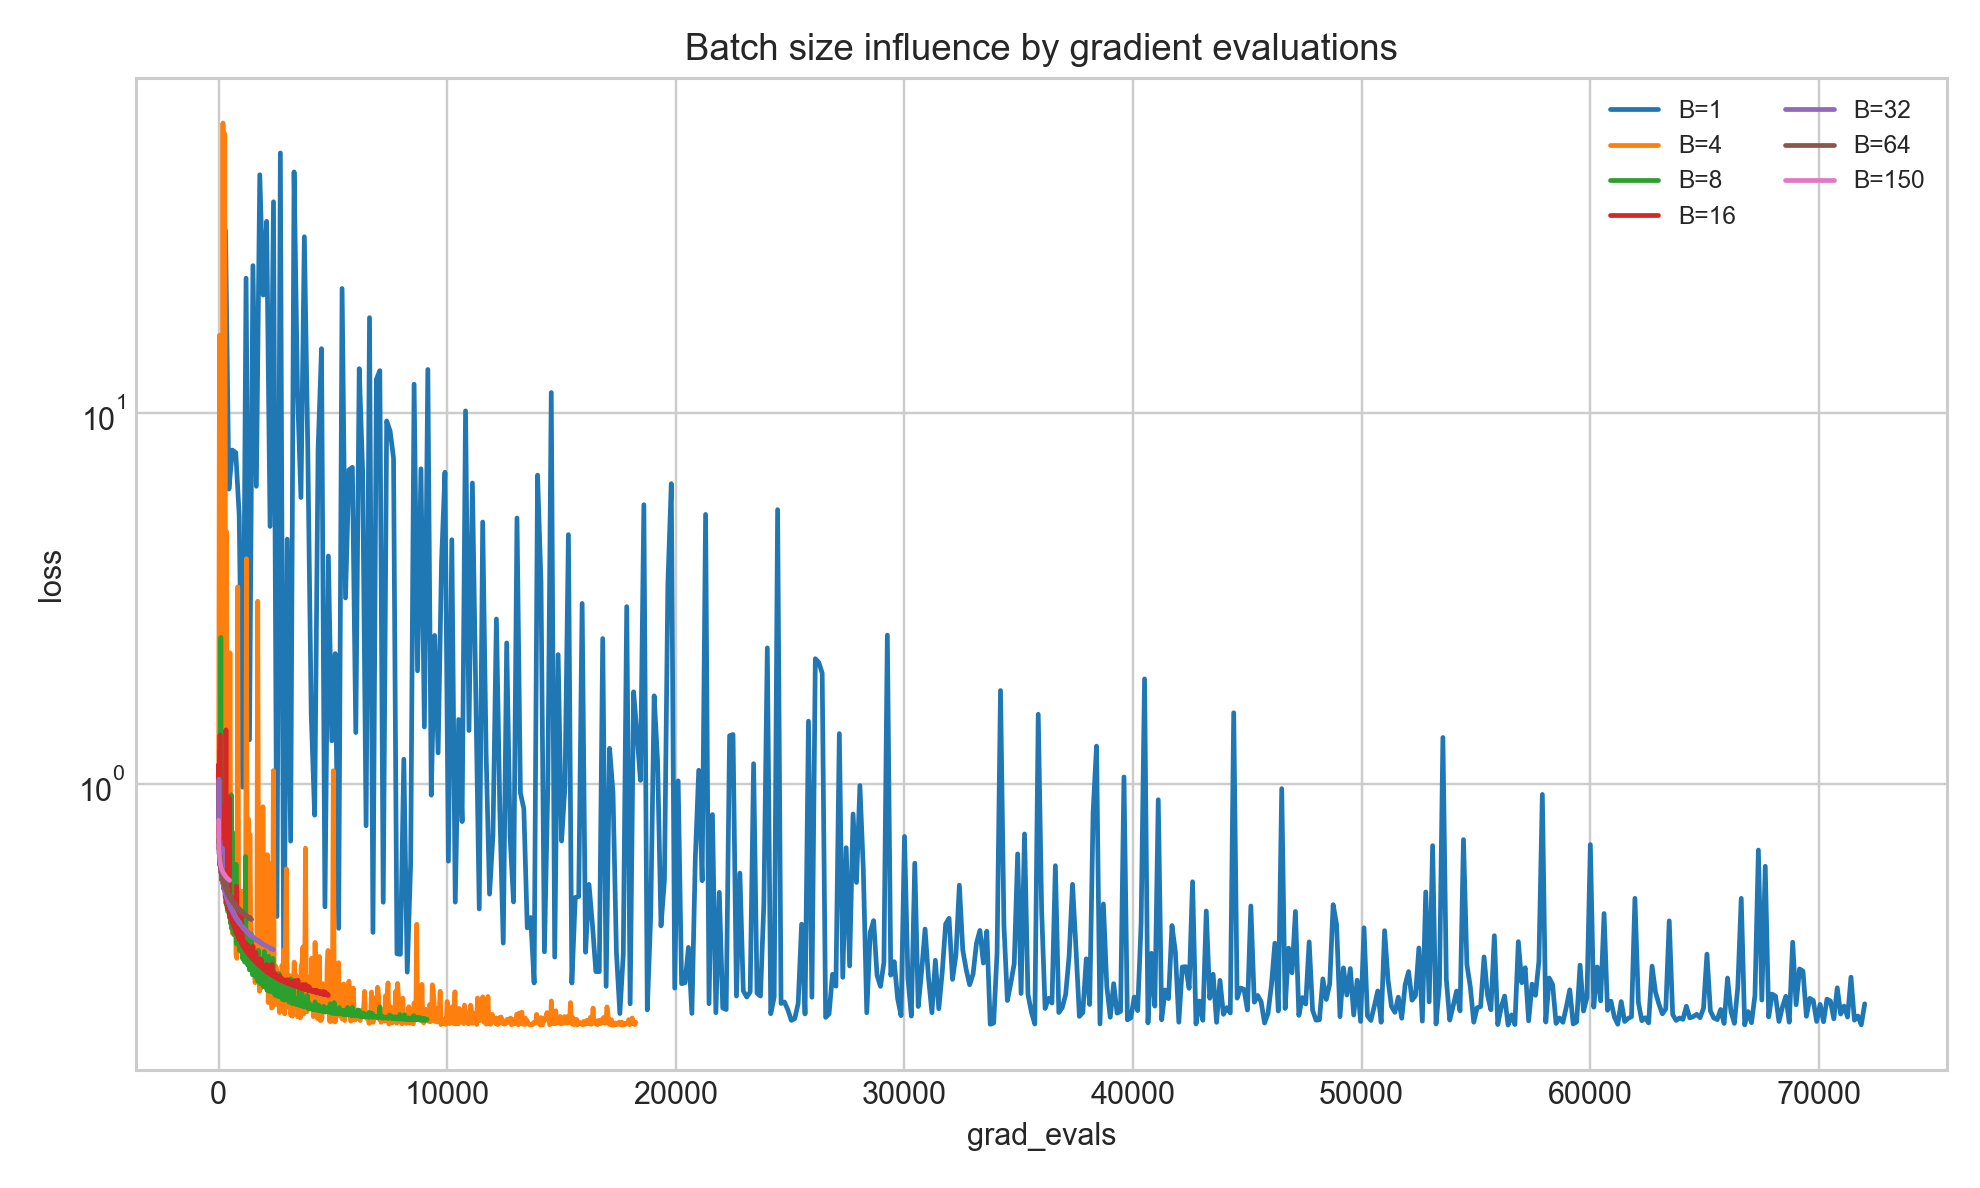
\includegraphics[width=0.85\textwidth]{batch_size/loss_by_grad_evals.png}
\caption{Потери по числу вычислений градиента для разных размеров батча}
\end{figure}

\subsection{Регуляризация}

\textbf{Зачем этот эксперимент.} Полином степени 10 имеет 11 параметров на 150 точек~--- модель достаточно гибкая для переобучения. Без регуляризации полином может <<колебаться>> между точками, давая большие значения вне данных. Задание требует:
\begin{itemize}
    \item для L1, L2 и Elastic Net рассмотреть несколько значений $\lambda$;
    \item построить графики динамики полного loss, эмпирического риска и регуляризационных слагаемых;
    \item сравнить коэффициенты моделей до и после регуляризации;
    \item сделать вывод о влиянии разных типов регуляризации на качество и структуру модели.
\end{itemize}

Эксперимент на наборе <<nonlinear>> со степенью 10 (mini-batch GD, batch\_size = 32, 1000 эпох).

\begin{table}[H]
\centering
\caption{Влияние регуляризации (степень 10, nonlinear)}
\begin{adjustbox}{max width=\textwidth}
\begin{tabular}{llccccc}
\toprule
\textbf{Тип} & $\lambda$ & \textbf{Loss} & \textbf{MSE (risk)} & \textbf{L1-штраф} & \textbf{L2-штраф} & \textbf{Clipped} \\
\midrule
none & --- & 0.4006 & 0.4006 & 0 & 0 & 727 \\
\midrule
L1 & $10^{-4}$ & 0.4000 & 0.3998 & 0.00012 & 0 & 696 \\
L1 & $10^{-3}$ & 0.3974 & 0.3962 & 0.00125 & 0 & 705 \\
L1 & $10^{-2}$ & 0.4218 & 0.4110 & 0.01084 & 0 & 722 \\
L1 & $10^{-1}$ & 0.5292 & 0.4570 & 0.07224 & 0 & 756 \\
\midrule
L2 & $10^{-4}$ & 0.3993 & 0.3992 & 0 & 0.00002 & 686 \\
L2 & $10^{-3}$ & 0.3993 & 0.3991 & 0 & 0.00019 & 716 \\
L2 & $10^{-2}$ & 0.4105 & 0.4088 & 0 & 0.00174 & 727 \\
L2 & $10^{-1}$ & 0.4472 & 0.4303 & 0 & 0.01689 & 766 \\
\midrule
ElasticNet & $10^{-3}$ & 0.4048 & 0.4034 & 0.00119 & 0.00018 & 715 \\
ElasticNet & $10^{-1}$ & 0.5166 & 0.4404 & 0.06875 & 0.00744 & 700 \\
\bottomrule
\end{tabular}
\end{adjustbox}
\end{table}

Лучший MSE (0.396) достигается при L1 с $\lambda_1 = 10^{-3}$. Слишком сильная регуляризация ($\lambda = 0.1$) приводит к underfitting. L2 с малыми $\lambda$ мало влияет на MSE, но стабилизирует обучение.

\begin{figure}[H]
\centering
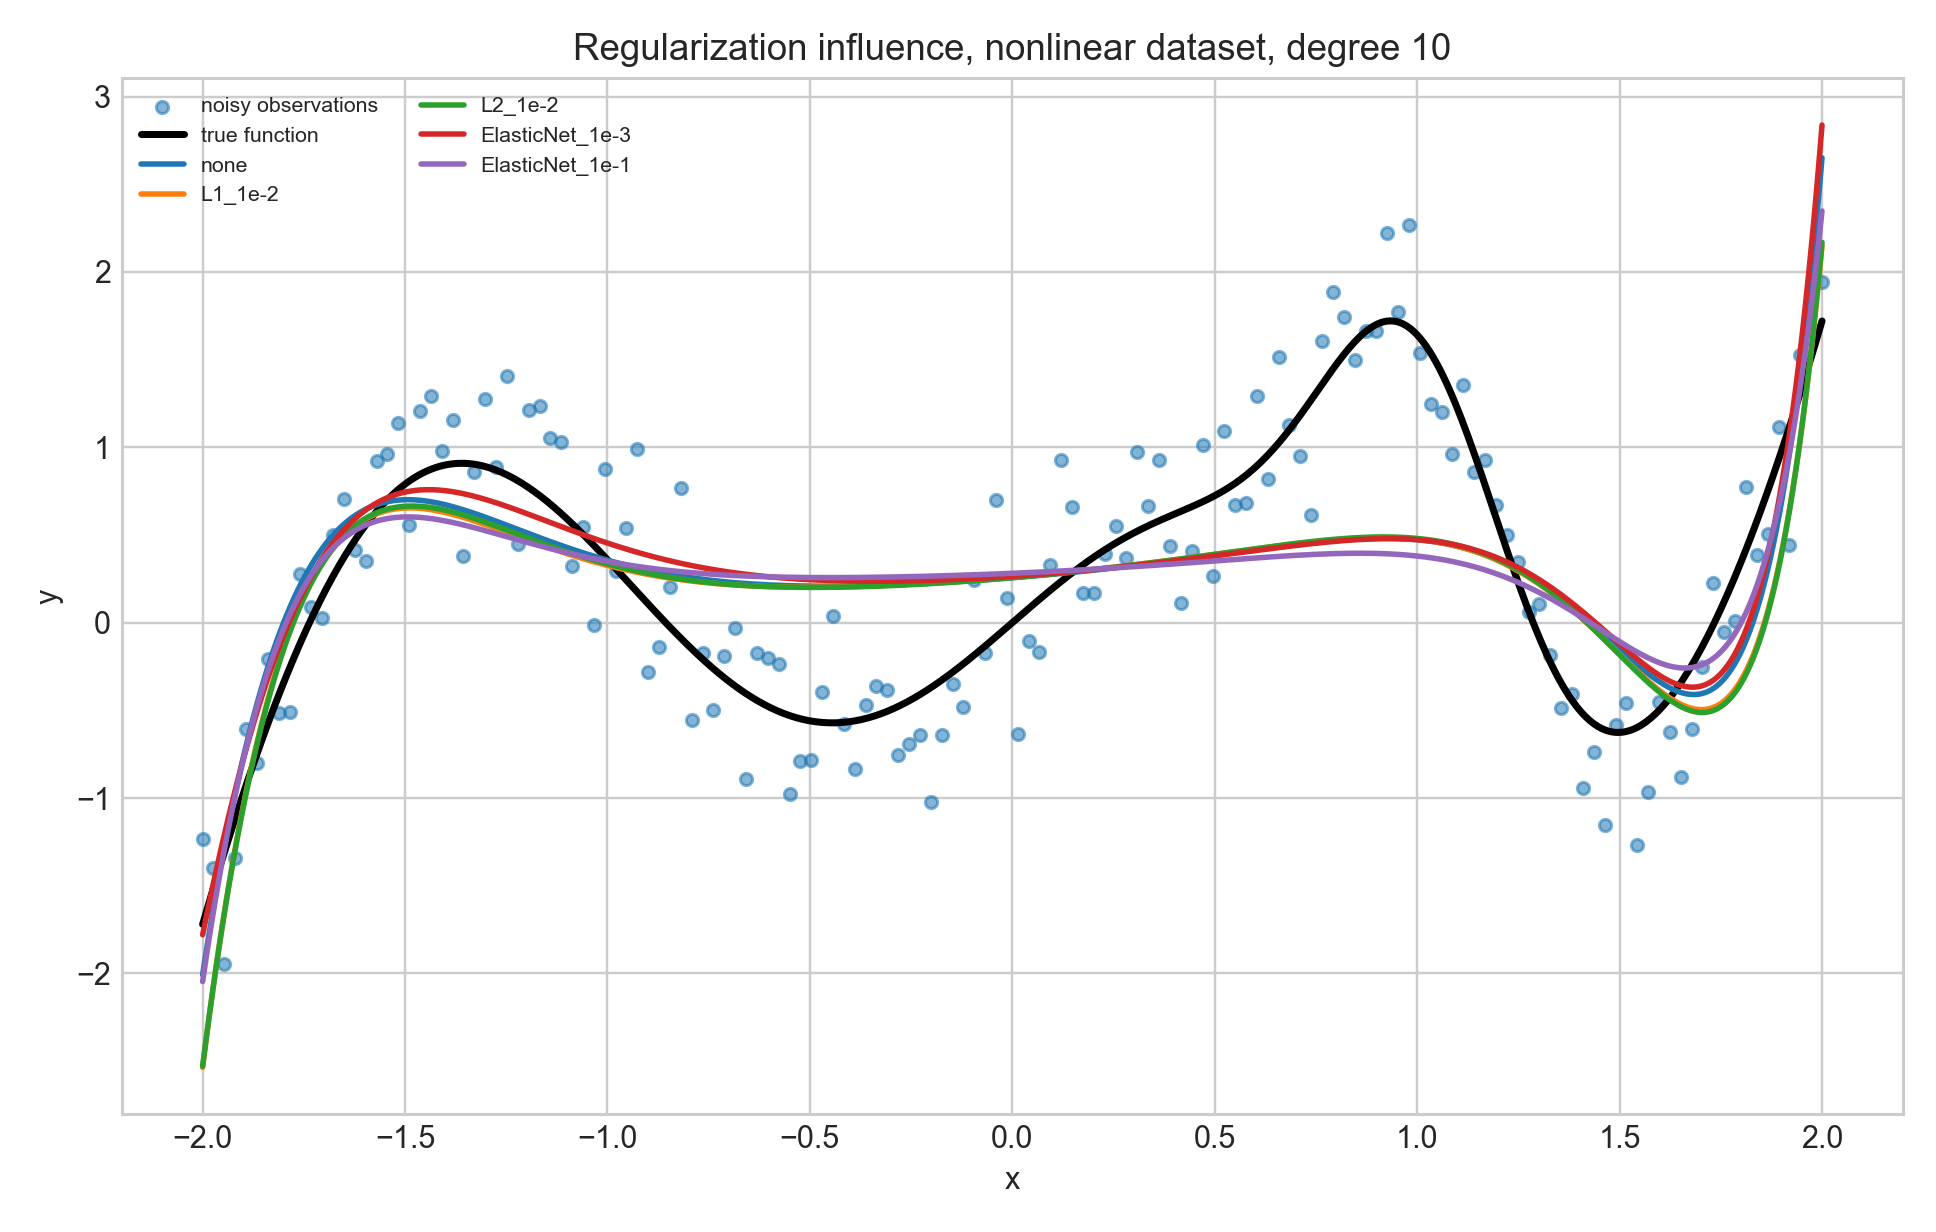
\includegraphics[width=0.85\textwidth]{regularization/fits_selected.png}
\caption{Аппроксимация при разных типах регуляризации}
\end{figure}

\begin{figure}[H]
\centering
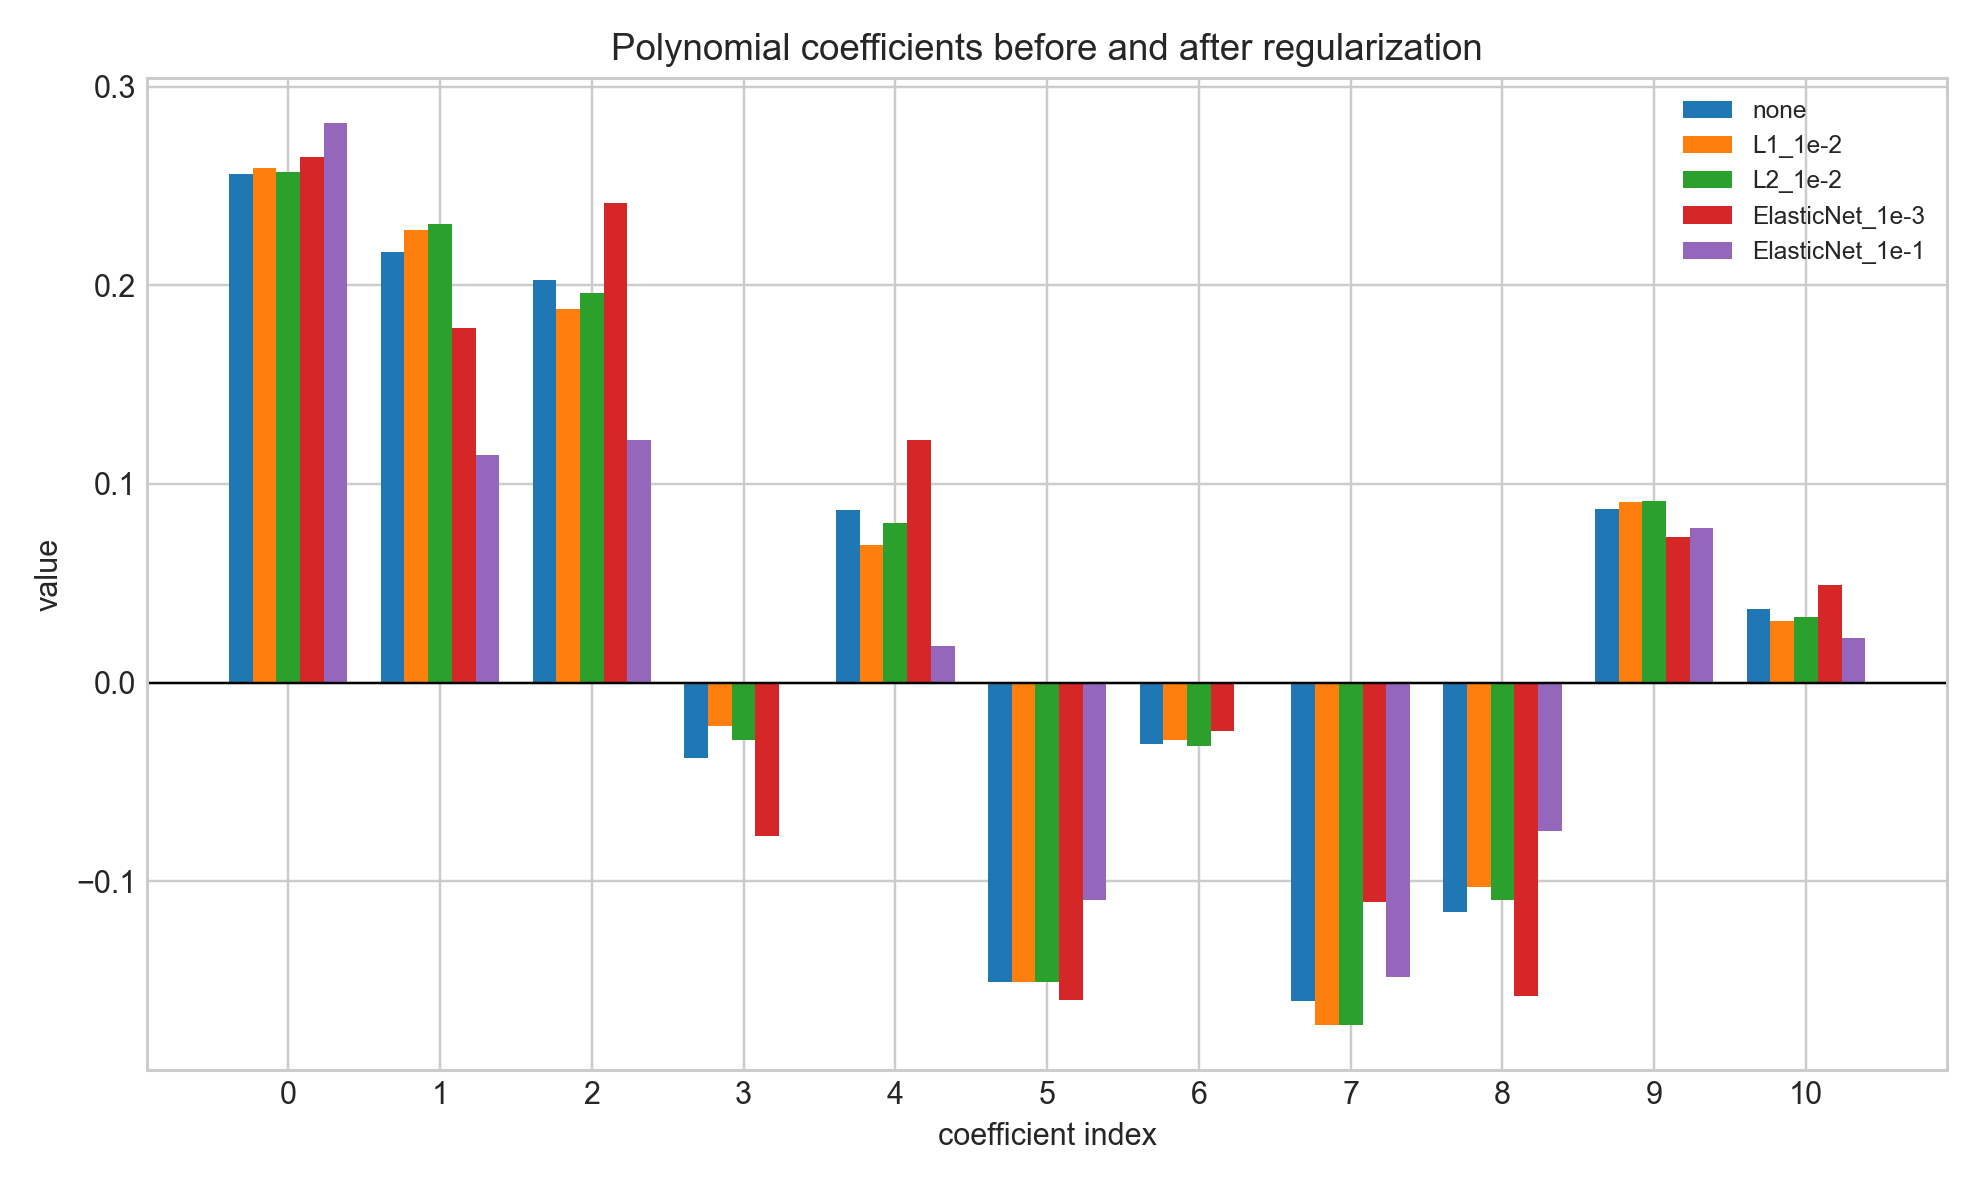
\includegraphics[width=0.85\textwidth]{regularization/coefficients_selected.png}
\caption{Коэффициенты полинома при разных типах регуляризации}
\end{figure}

\begin{figure}[H]
\centering
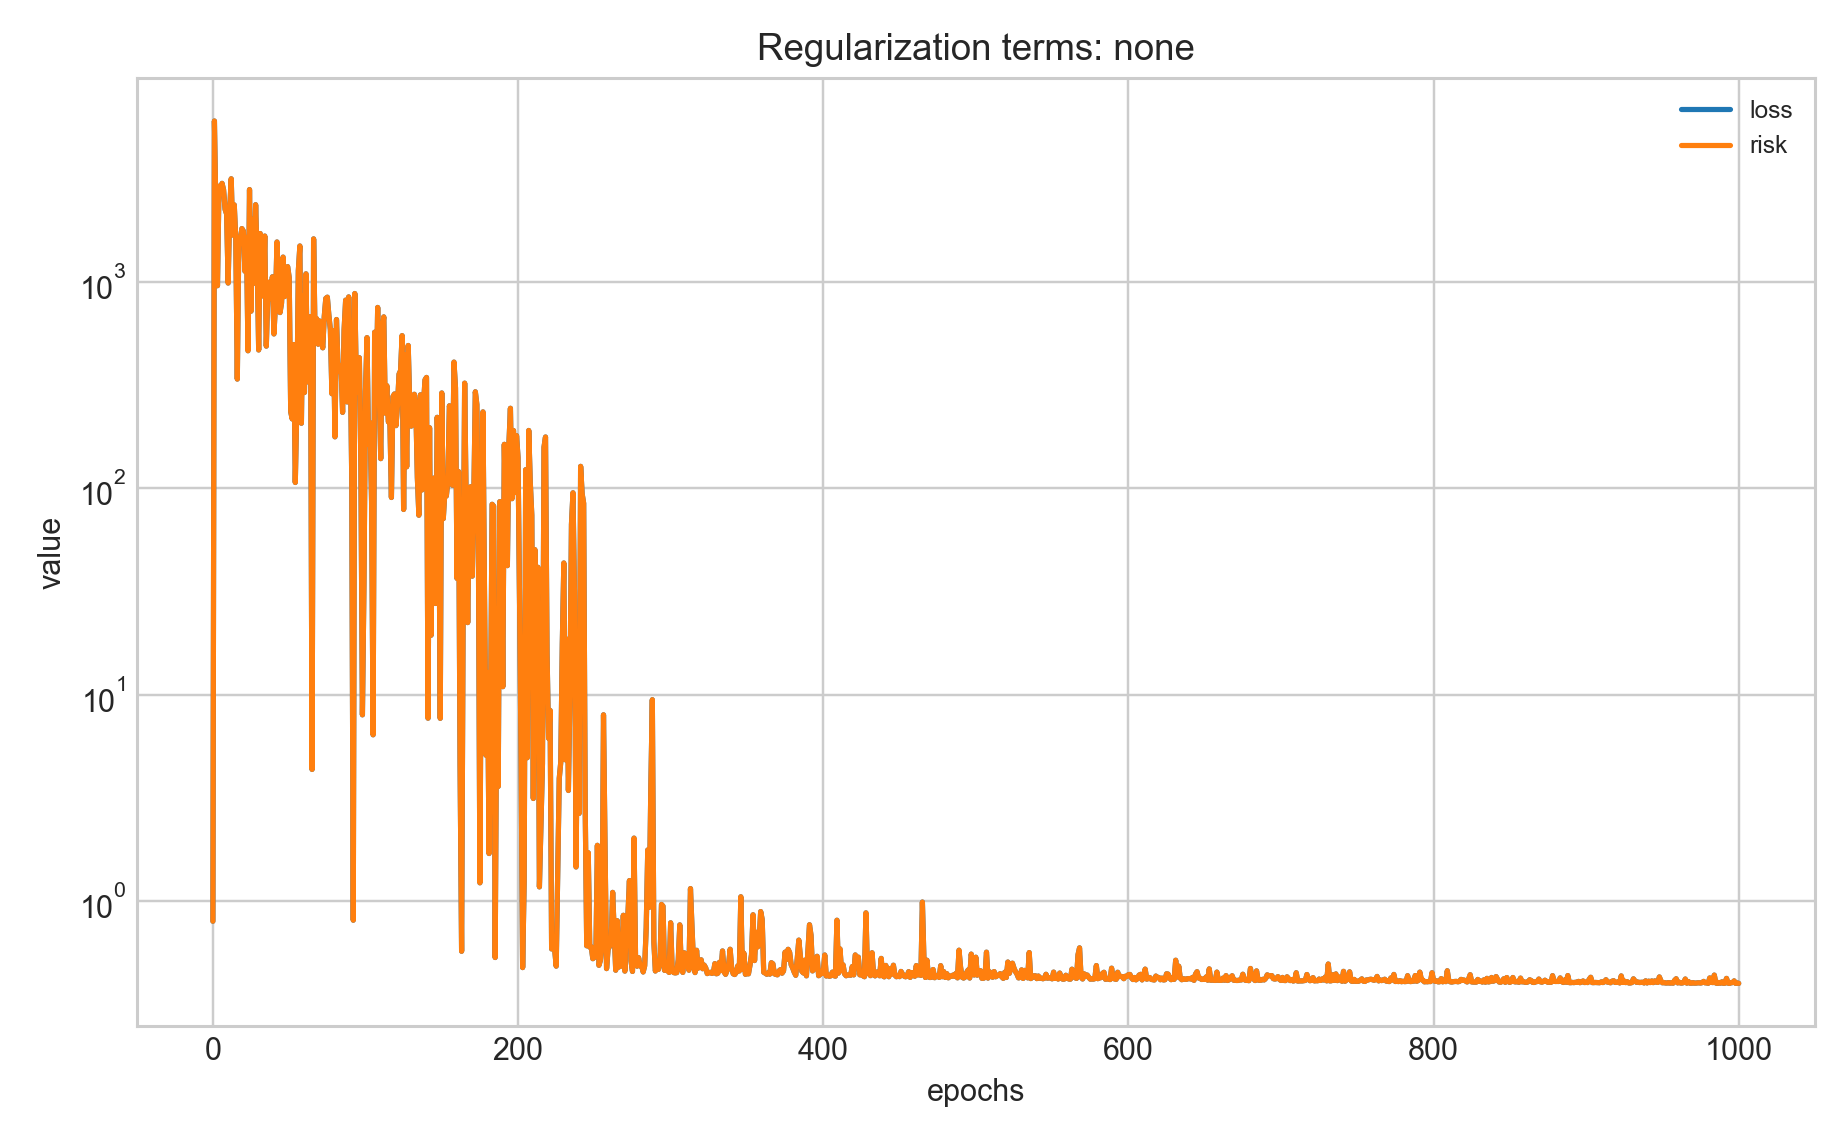
\includegraphics[width=0.48\textwidth]{regularization/terms_none.png}
\hfill
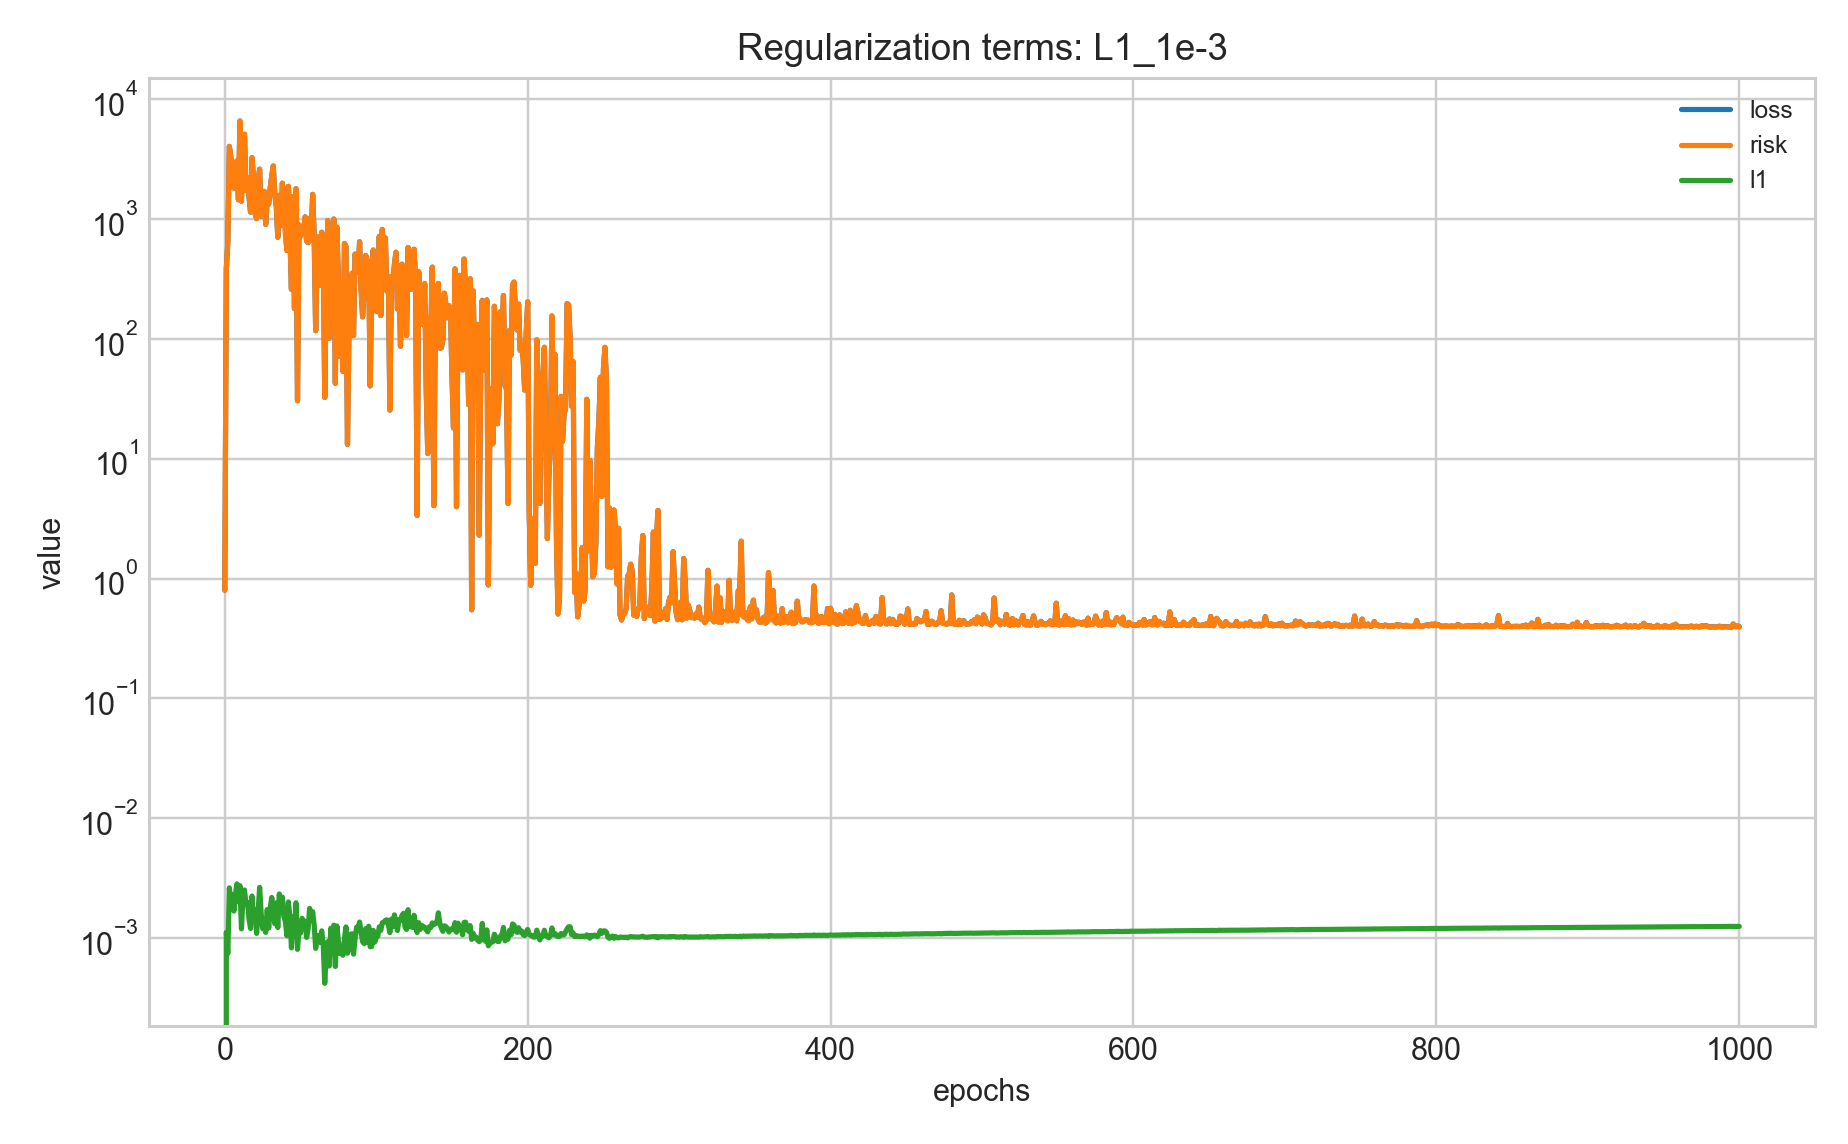
\includegraphics[width=0.48\textwidth]{regularization/terms_l1_1e-3.png}
\caption{Компоненты потерь: без регуляризации (слева) и L1 $\lambda=10^{-3}$ (справа)}
\end{figure}

\begin{figure}[H]
\centering
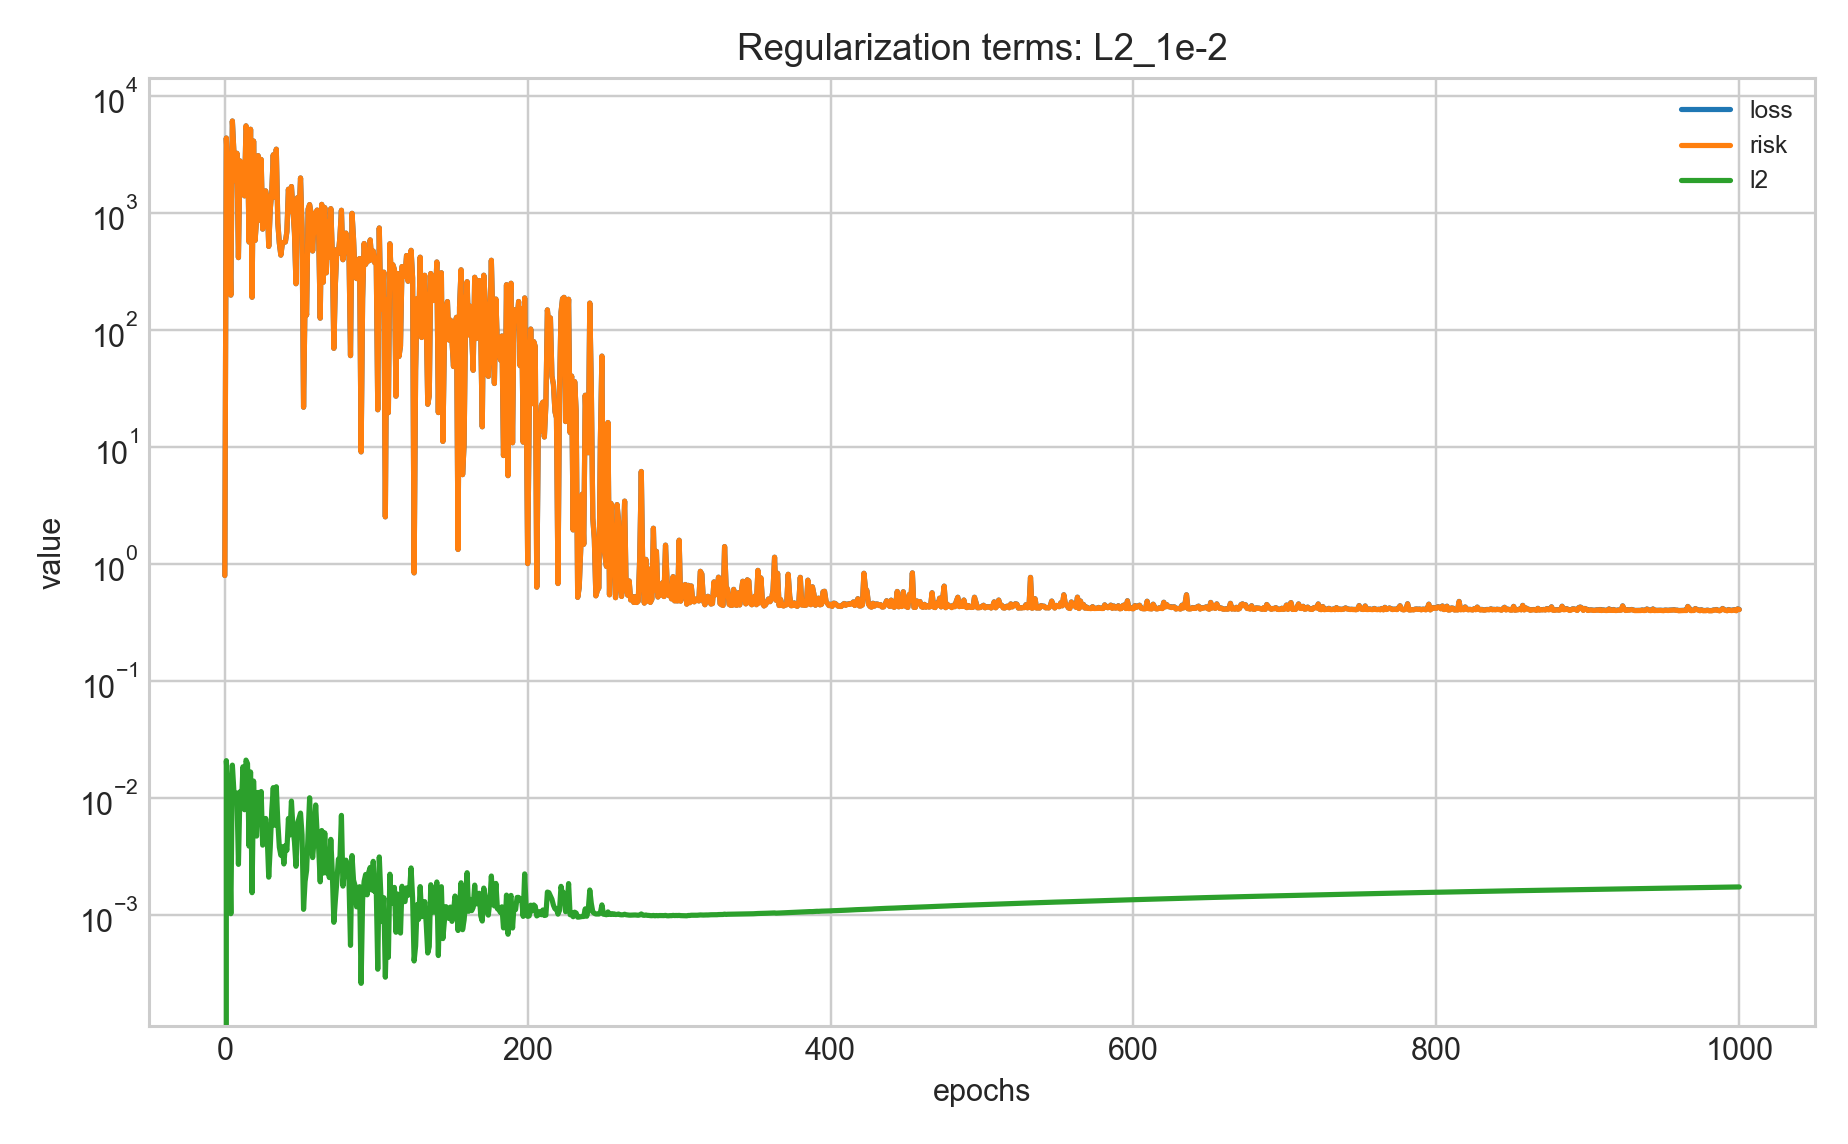
\includegraphics[width=0.48\textwidth]{regularization/terms_l2_1e-2.png}
\hfill
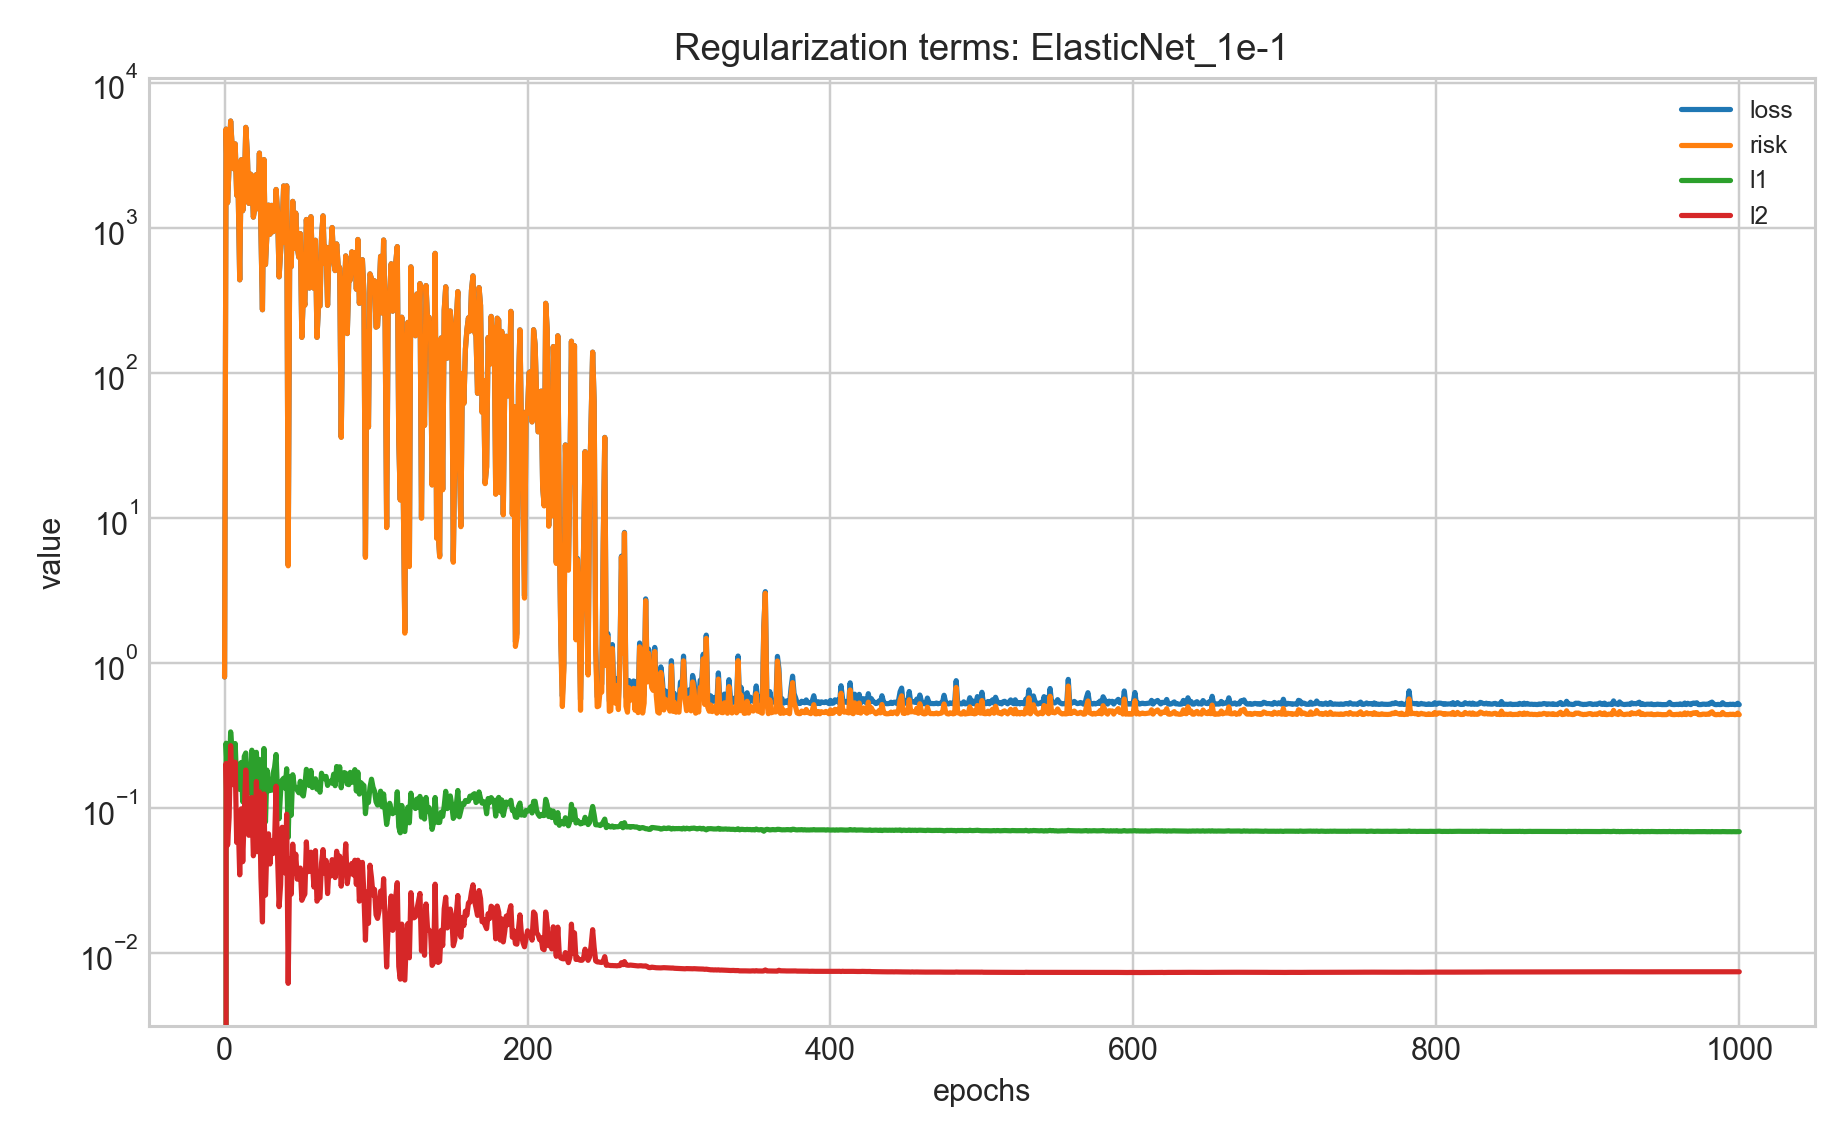
\includegraphics[width=0.48\textwidth]{regularization/terms_elasticnet_1e-1.png}
\caption{Компоненты потерь: L2 $\lambda=10^{-2}$ (слева) и ElasticNet $\lambda=10^{-1}$ (справа)}
\end{figure}

\subsection{Gauss-Newton vs Levenberg-Marquardt на плохо обусловленной задаче}

\textbf{Зачем этот эксперимент.} Задание требует отдельно сравнить GN и LM на нелинейной или плохо обусловленной постановке. При степени 10 без нормализации признаков число обусловленности $\kappa(\Phi^T\Phi) \sim 3 \cdot 10^7$, что делает решение нормальных уравнений численно нестабильным. Gauss-Newton может <<промахнуться>> из-за ошибок округления, а Levenberg-Marquardt остаётся устойчивым: демпфирование $\mu I$ регуляризует матрицу, обеспечивая $\kappa(\Phi^T\Phi + \mu I) \leq \kappa(\Phi^T\Phi) / \mu \cdot \lambda_{\min}$.

\begin{figure}[H]
\centering
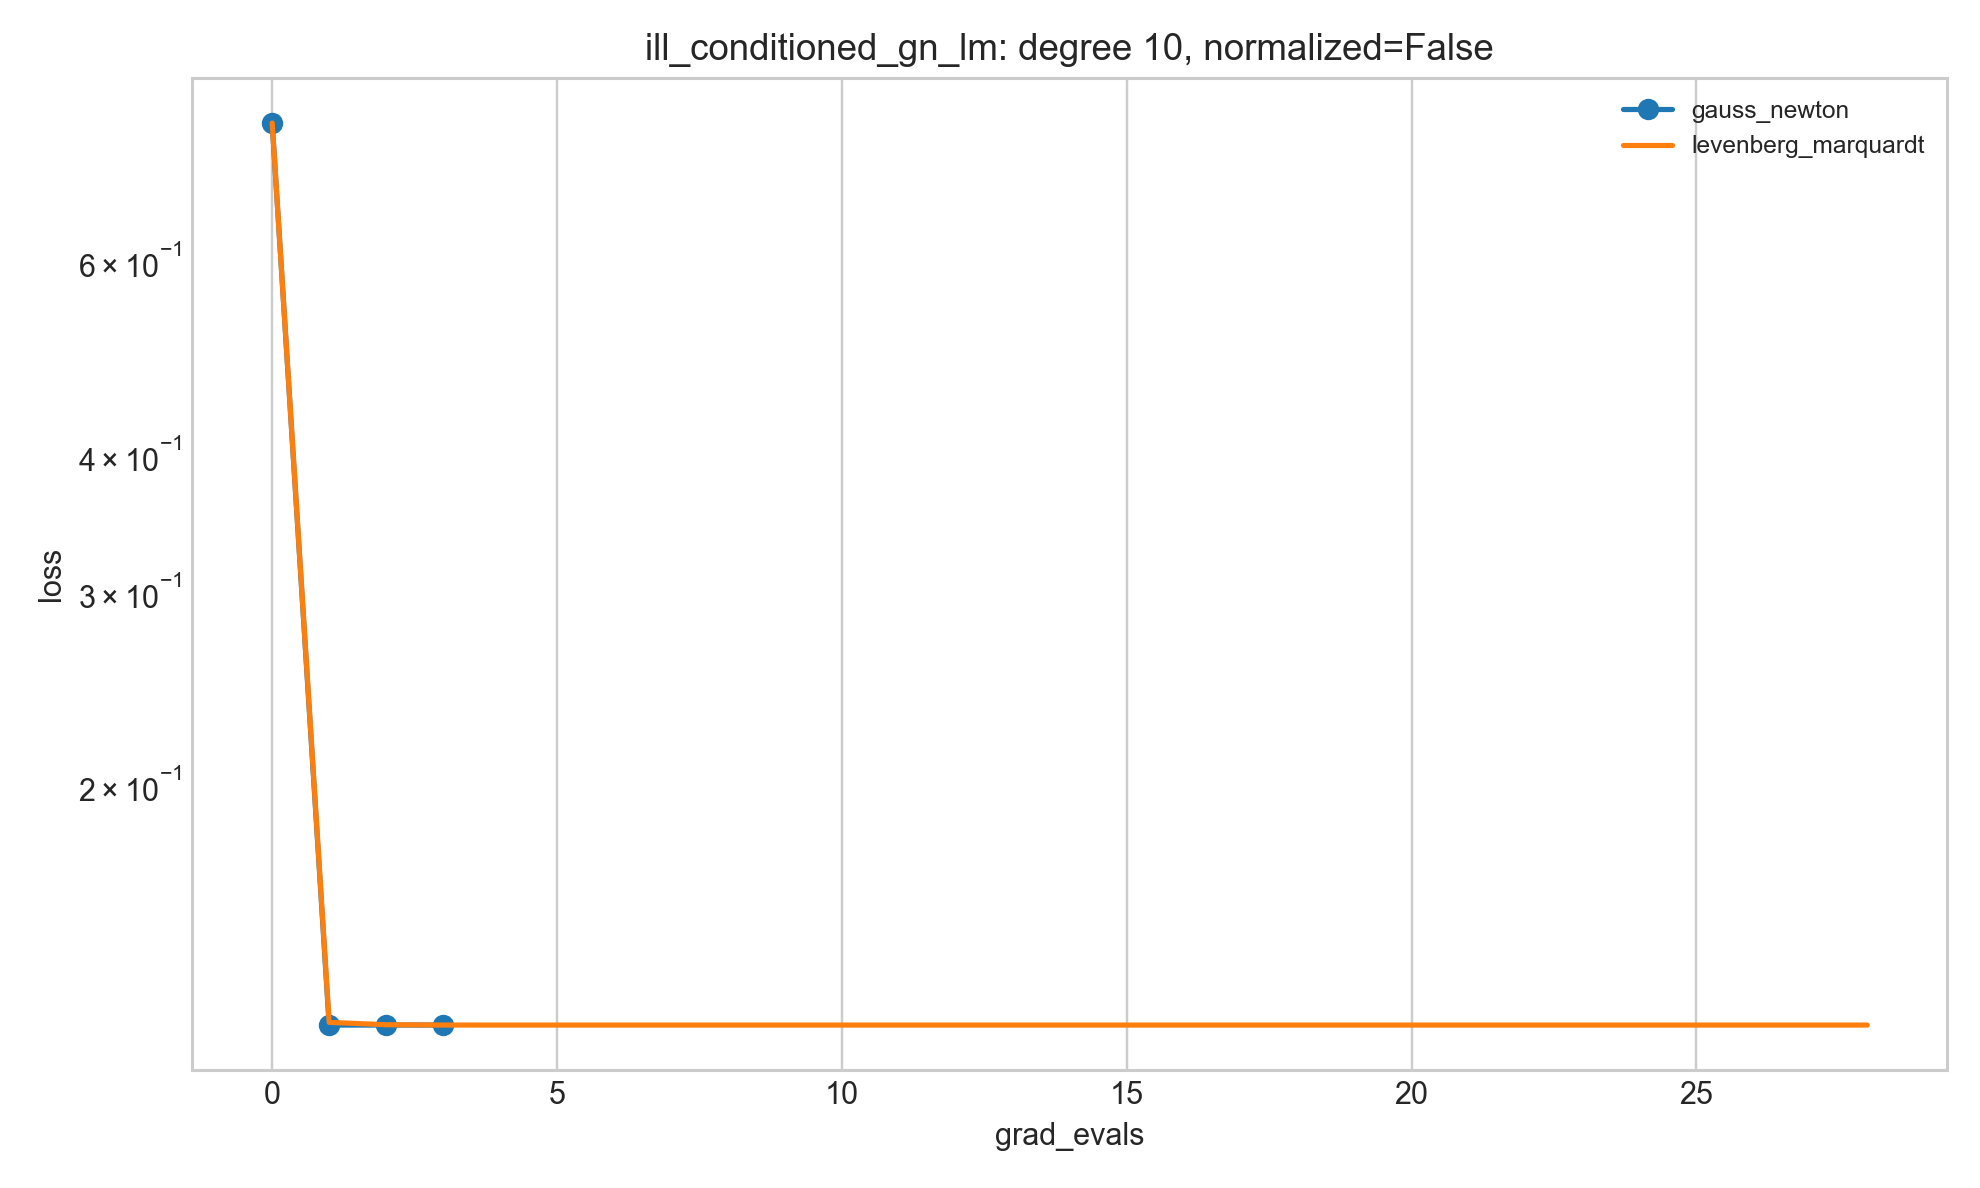
\includegraphics[width=0.85\textwidth]{ill_conditioned_gn_lm/loss_degree_10_normalized_False.png}
\caption{GN vs LM: потери на плохо обусловленной задаче (степень 10, без нормализации)}
\end{figure}

%=============================================================================
\section{Сравнение методов}

\begin{table}[H]
\centering
\caption{Сравнительная характеристика методов оптимизации для регрессии}
\begin{adjustbox}{max width=\textwidth}
\begin{tabular}{lccl}
\toprule
\textbf{Метод} & \textbf{Итер. до сход.} & \textbf{Сложность итерации} & \textbf{Особенности} \\
\midrule
Analytic & 1 & $O(n^2 m)$ & только степень 1 \\
SGD & $>$360 & $O(n)$ & шумная сходимость \\
Mini-batch & $>$360 & $O(Bn)$ & баланс скорость/шум \\
Gauss-Newton & 2 & $O(n^2 m + n^3)$ & требует $\Phi^T\Phi$ обратима \\
Lev.-Marq. & 4--25 & $O(n^2 m + n^3)$ & устойчивее GN \\
\bottomrule
\end{tabular}
\end{adjustbox}
\end{table}

%=============================================================================
\section{Выводы}

\subsection*{Сравнение методов оптимизации}

\begin{enumerate}
    \item \textbf{Gauss-Newton}~--- безусловный лидер по скорости сходимости: 2 итерации для любой степени полинома при нормализованных признаках. Для линейных наименьших квадратов задача решается точно за один шаг решения нормальных уравнений.

    \item \textbf{Levenberg-Marquardt} сходится за 4--7 итераций в большинстве случаев. На нелинейном наборе при степени 4 LM потребовал 25 итераций (18 отклонённых шагов), что связано с плохой начальной точкой и необходимостью увеличения $\mu$ до 40.96. На ненормализованных признаках степени 10 LM стабильно работает благодаря демпфированию $\mu I$.

    \item \textbf{SGD и mini-batch GD} не сходятся за 360 эпох, но достигают приемлемых значений MSE при малых степенях. При степени 5 на нелинейном наборе SGD (MSE = 0.239) приближается к оптимуму Gauss-Newton (0.225), тогда как mini-batch с batch\_size = 32 значительно отстаёт (MSE = 0.367).
\end{enumerate}

\subsection*{Медленная сходимость и чувствительность}

\begin{itemize}
    \item \textbf{SGD при высоких степенях} демонстрирует медленную сходимость: при степени 5 на наборе almost\_linear происходит 578 обрезок градиента (gradient clipping), что указывает на нестабильность обновлений. Число обусловленности матрицы признаков при степени 5 составляет $\sim 1390$.

    \item \textbf{Mini-batch при больших batch\_size}: при batch\_size = 150 (почти полный GD) за 480 эпох достигается MSE = 0.552 vs 0.229 при batch\_size = 4. Крупные батчи медленнее исследуют пространство параметров, т.к. делают меньше обновлений за эпоху.

    \item \textbf{Gauss-Newton на плохо обусловленной задаче}: без нормализации число обусловленности $\Phi^T\Phi$ при степени 10 составляет $\sim 3 \cdot 10^7$, что приводит к потере точности при решении системы нормальных уравнений.
\end{itemize}

\subsection*{Влияние регуляризации на структуру коэффициентов}

\begin{itemize}
    \item \textbf{L1 ($\lambda=10^{-3}$)} улучшает MSE с 0.401 до 0.396 при степени 10 за счёт обнуления шумных коэффициентов высоких степеней. При $\lambda=0.1$ коэффициенты $w_4, w_7$ практически обнуляются ($\sim 10^{-4}$), но наступает underfitting (MSE = 0.457).

    \item \textbf{L2} уменьшает абсолютные значения всех коэффициентов равномерно, не создавая разреженности. При $\lambda=10^{-4}$ влияние минимально (L2-штраф $= 2 \cdot 10^{-5}$).

    \item \textbf{ElasticNet} комбинирует свойства L1 и L2: при $\lambda_1 = \lambda_2 = 0.1$ коэффициенты уменьшены и частично обнулены (MSE = 0.440).
\end{itemize}

\subsection*{Нормализация признаков}

Нормализация критически важна: число обусловленности матрицы $\Phi$ при степени 10 составляет $\sim 3 \cdot 10^7$. Без нормализации стохастические методы нестабильны, а Gauss-Newton теряет точность при решении нормальных уравнений. Levenberg-Marquardt устойчивее благодаря регуляризующему эффекту демпфирования.

\end{document}
